\documentclass[a4paper]{book}
\usepackage{a4wide}
\usepackage{makeidx}
\usepackage{fancyhdr}
\usepackage{graphicx}
\usepackage{multicol}
\usepackage{float}
\usepackage{textcomp}
\usepackage{alltt}
\usepackage{times}
\usepackage{ifpdf}
\ifpdf
\usepackage[pdftex,
            pagebackref=true,
            colorlinks=true,
            linkcolor=blue,
            unicode
           ]{hyperref}
\else
\usepackage[ps2pdf,
            pagebackref=true,
            colorlinks=true,
            linkcolor=blue,
            unicode
           ]{hyperref}
\usepackage{pspicture}
\fi
\usepackage[utf8]{inputenc}
\usepackage{doxygen}
\makeindex
\setcounter{tocdepth}{3}
\renewcommand{\footrulewidth}{0.4pt}
\begin{document}
\begin{titlepage}
\vspace*{7cm}
\begin{center}
{\Large SFML Gui \\[1ex]\large 0.1 }\\
\vspace*{1cm}
{\large Generated by Doxygen 1.5.6}\\
\vspace*{0.5cm}
{\small Sun Jan 4 18:39:39 2009}\\
\end{center}
\end{titlepage}
\clearemptydoublepage
\pagenumbering{roman}
\tableofcontents
\clearemptydoublepage
\pagenumbering{arabic}
\chapter{Namespace Index}
\section{Namespace List}
Here is a list of all namespaces with brief descriptions:\begin{CompactList}
\item\contentsline{section}{\hyperlink{namespacesfgui}{sfgui} (All graphics widgets )}{\pageref{namespacesfgui}}{}
\end{CompactList}

\chapter{Class Index}
\section{Class Hierarchy}
This inheritance list is sorted roughly, but not completely, alphabetically:\begin{CompactList}
\item \contentsline{section}{sfgui::Error}{\pageref{classsfgui_1_1Error}}{}
\item \contentsline{section}{sfgui::Margin}{\pageref{structsfgui_1_1Margin}}{}
\item \contentsline{section}{sfgui::Object}{\pageref{classsfgui_1_1Object}}{}
\begin{CompactList}
\item \contentsline{section}{sfgui::Button}{\pageref{classsfgui_1_1Button}}{}
\item \contentsline{section}{sfgui::Checkbox}{\pageref{classsfgui_1_1Checkbox}}{}
\item \contentsline{section}{sfgui::TextEdit}{\pageref{classsfgui_1_1TextEdit}}{}
\item \contentsline{section}{Slider}{\pageref{classSlider}}{}
\item \contentsline{section}{Tooltip}{\pageref{classTooltip}}{}
\end{CompactList}
\end{CompactList}

\chapter{Class Index}
\section{Class List}
Here are the classes, structs, unions and interfaces with brief descriptions:\begin{CompactList}
\item\contentsline{section}{\hyperlink{classsfgui_1_1Button}{sfgui::Button} (A push button )}{\pageref{classsfgui_1_1Button}}{}
\item\contentsline{section}{\hyperlink{classsfgui_1_1Checkbox}{sfgui::Checkbox} (Class which provides checkbox buttons )}{\pageref{classsfgui_1_1Checkbox}}{}
\item\contentsline{section}{\hyperlink{classsfgui_1_1Error}{sfgui::Error} (\hyperlink{classsfgui_1_1Error}{Error} object. Inherited from std::exception )}{\pageref{classsfgui_1_1Error}}{}
\item\contentsline{section}{\hyperlink{structsfgui_1_1Margin}{sfgui::Margin} (Struct which contains margin values )}{\pageref{structsfgui_1_1Margin}}{}
\item\contentsline{section}{\hyperlink{classsfgui_1_1Object}{sfgui::Object} (A simple graphic item )}{\pageref{classsfgui_1_1Object}}{}
\item\contentsline{section}{\hyperlink{classSlider}{Slider} }{\pageref{classSlider}}{}
\item\contentsline{section}{\hyperlink{classsfgui_1_1TextEdit}{sfgui::TextEdit} (A single line text entry )}{\pageref{classsfgui_1_1TextEdit}}{}
\end{CompactList}

\chapter{File Index}
\section{File List}
Here is a list of all files with brief descriptions:\begin{CompactList}
\item\contentsline{section}{\hyperlink{button_8cpp}{button.cpp} }{\pageref{button_8cpp}}{}
\item\contentsline{section}{\hyperlink{button_8hpp}{button.hpp} }{\pageref{button_8hpp}}{}
\item\contentsline{section}{\hyperlink{constantes_8hpp}{constantes.hpp} (Description not set )}{\pageref{constantes_8hpp}}{}
\item\contentsline{section}{\hyperlink{error_8hpp}{error.hpp} }{\pageref{error_8hpp}}{}
\item\contentsline{section}{\hyperlink{main_8cpp}{main.cpp} }{\pageref{main_8cpp}}{}
\item\contentsline{section}{\hyperlink{margin_8cpp}{margin.cpp} }{\pageref{margin_8cpp}}{}
\item\contentsline{section}{\hyperlink{margin_8hpp}{margin.hpp} (A simple struct for margin )}{\pageref{margin_8hpp}}{}
\item\contentsline{section}{\hyperlink{object_8cpp}{object.cpp} }{\pageref{object_8cpp}}{}
\item\contentsline{section}{\hyperlink{object_8hpp}{object.hpp} }{\pageref{object_8hpp}}{}
\item\contentsline{section}{\hyperlink{textedit_8cpp}{textedit.cpp} }{\pageref{textedit_8cpp}}{}
\item\contentsline{section}{\hyperlink{textedit_8hpp}{textedit.hpp} }{\pageref{textedit_8hpp}}{}
\end{CompactList}

\chapter{Namespace Documentation}
\hypertarget{namespacesfgui}{
\section{sfgui Namespace Reference}
\label{namespacesfgui}\index{sfgui@{sfgui}}
}
All graphics widgets.  


\subsection*{Classes}
\begin{CompactItemize}
\item 
class \hyperlink{classsfgui_1_1Button}{Button}
\begin{CompactList}\small\item\em A push button. \item\end{CompactList}\item 
class \hyperlink{classsfgui_1_1Error}{Error}
\item 
struct \hyperlink{structsfgui_1_1Margin}{Margin}
\begin{CompactList}\small\item\em Struct which contains margin values. \item\end{CompactList}\item 
class \hyperlink{classsfgui_1_1Object}{Object}
\begin{CompactList}\small\item\em A simple graphic item. \item\end{CompactList}\item 
class \hyperlink{classsfgui_1_1TextEdit}{TextEdit}
\begin{CompactList}\small\item\em A single line text entry. \item\end{CompactList}\end{CompactItemize}
\subsection*{Enumerations}
\begin{CompactItemize}
\item 
enum \{ \hyperlink{namespacesfgui_ed969f0aaa542b462035e828757f431328ce9405120beac8fae51bc232aeabec}{Left}, 
\hyperlink{namespacesfgui_ed969f0aaa542b462035e828757f4313d4fbbcf5a5a40412eeb0175f82c85b3f}{Right}, 
\hyperlink{namespacesfgui_ed969f0aaa542b462035e828757f43130172869b534ad2378e28e388342699cc}{Center}
 \}
\end{CompactItemize}


\subsection{Detailed Description}
All graphics widgets. 

This namespace contains all the graphics widgets 

\subsection{Enumeration Type Documentation}
\hypertarget{namespacesfgui_ed969f0aaa542b462035e828757f4313}{
\subsubsection["@0]{\setlength{\rightskip}{0pt plus 5cm}anonymous enum}}
\label{namespacesfgui_ed969f0aaa542b462035e828757f4313}


This enumeration defines the position of an item (such as text). It is used by widget to define autoposition (like \hyperlink{classsfgui_1_1Button}{Button} which has SetTextPosition...) \begin{Desc}
\item[Enumerator: ]\par
\begin{description}
\index{Left@{Left}!sfgui@{sfgui}}\index{sfgui@{sfgui}!Left@{Left}}\item[{\em 
\hypertarget{namespacesfgui_ed969f0aaa542b462035e828757f431328ce9405120beac8fae51bc232aeabec}{
Left}
\label{namespacesfgui_ed969f0aaa542b462035e828757f431328ce9405120beac8fae51bc232aeabec}
}]\hyperlink{classsfgui_1_1Object}{Object} is on the left. \index{Right@{Right}!sfgui@{sfgui}}\index{sfgui@{sfgui}!Right@{Right}}\item[{\em 
\hypertarget{namespacesfgui_ed969f0aaa542b462035e828757f4313d4fbbcf5a5a40412eeb0175f82c85b3f}{
Right}
\label{namespacesfgui_ed969f0aaa542b462035e828757f4313d4fbbcf5a5a40412eeb0175f82c85b3f}
}]\hyperlink{classsfgui_1_1Object}{Object} is on the right. \index{Center@{Center}!sfgui@{sfgui}}\index{sfgui@{sfgui}!Center@{Center}}\item[{\em 
\hypertarget{namespacesfgui_ed969f0aaa542b462035e828757f43130172869b534ad2378e28e388342699cc}{
Center}
\label{namespacesfgui_ed969f0aaa542b462035e828757f43130172869b534ad2378e28e388342699cc}
}]\hyperlink{classsfgui_1_1Object}{Object} is centered. \end{description}
\end{Desc}


\chapter{Class Documentation}
\hypertarget{classsfgui_1_1Button}{
\section{sfgui::Button Class Reference}
\label{classsfgui_1_1Button}\index{sfgui::Button@{sfgui::Button}}
}
A push button.  


{\tt \#include $<$button.hpp$>$}

Inheritance diagram for sfgui::Button:\nopagebreak
\begin{figure}[H]
\begin{center}
\leavevmode
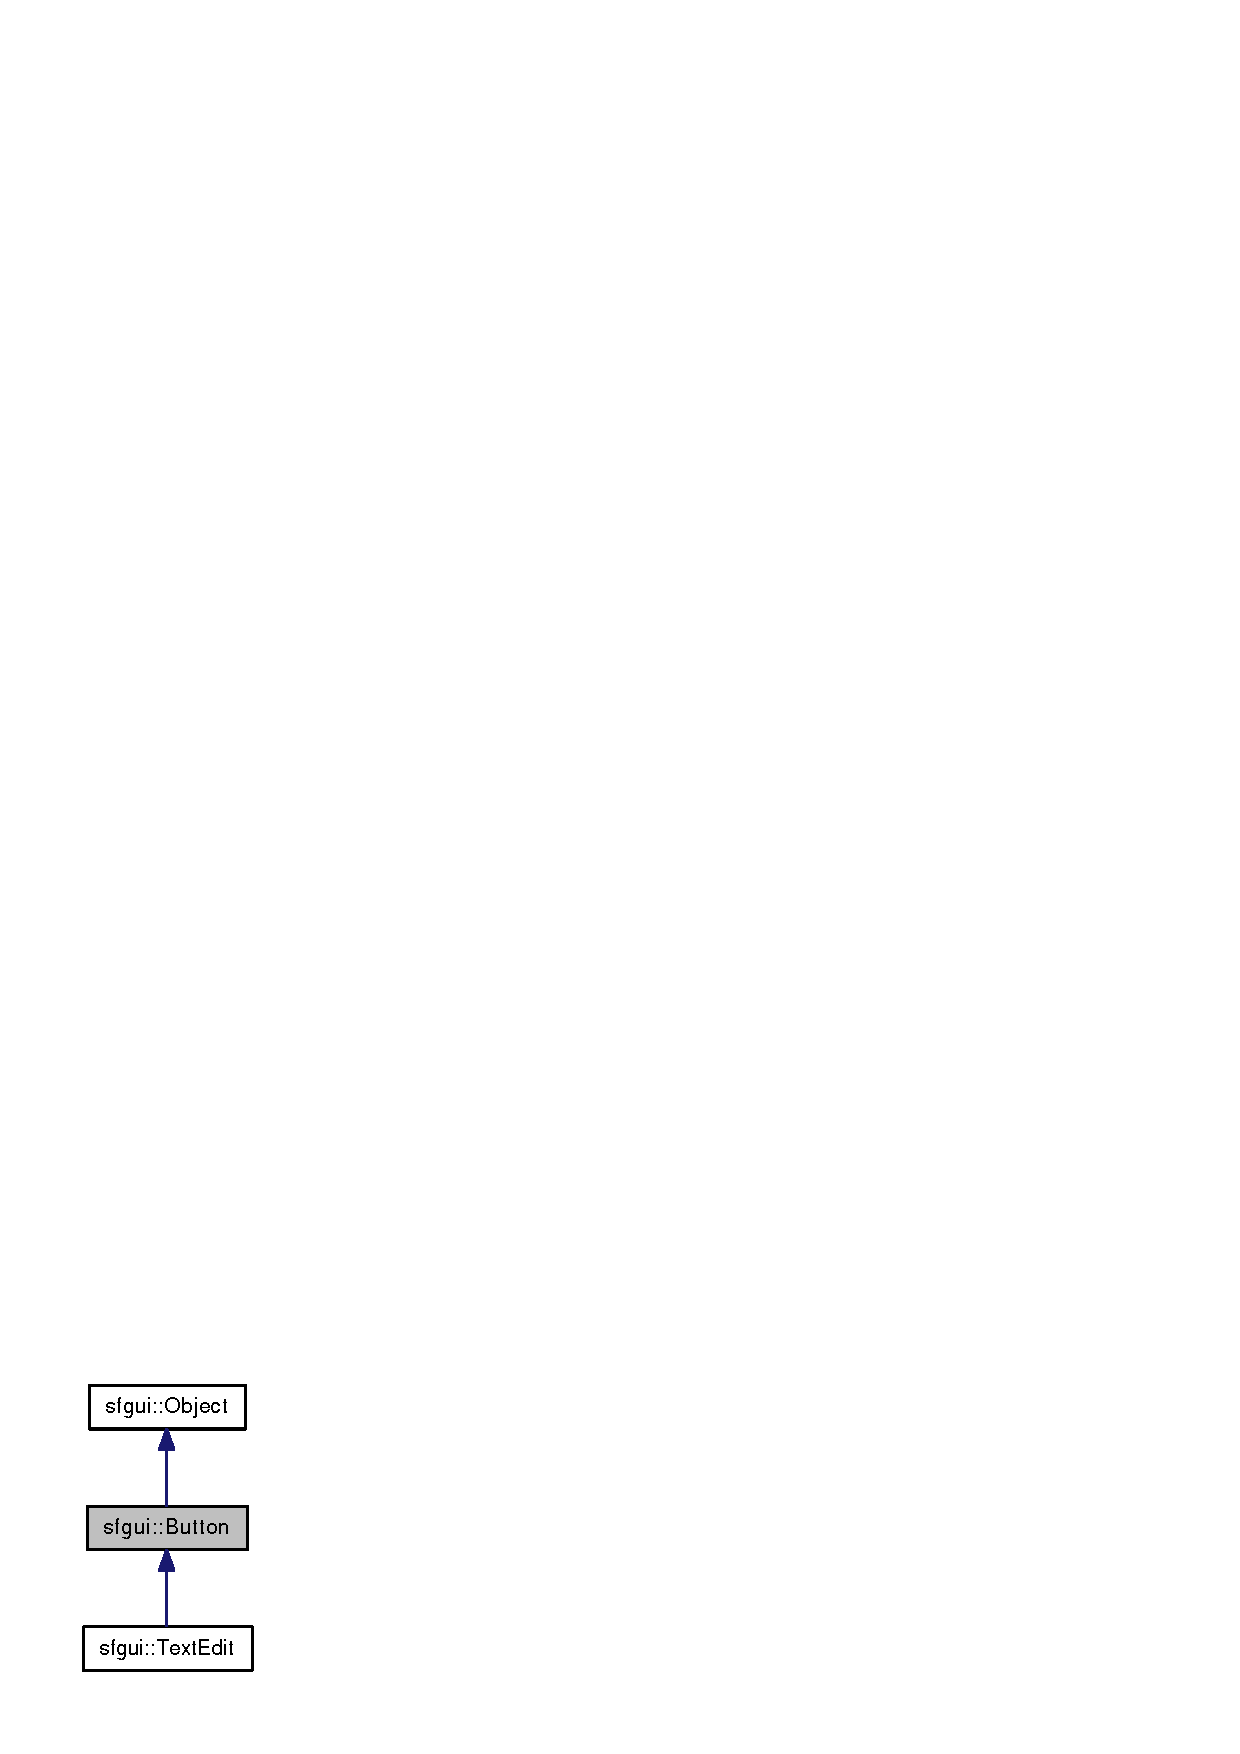
\includegraphics[width=62pt]{classsfgui_1_1Button__inherit__graph}
\end{center}
\end{figure}
Collaboration diagram for sfgui::Button:\nopagebreak
\begin{figure}[H]
\begin{center}
\leavevmode
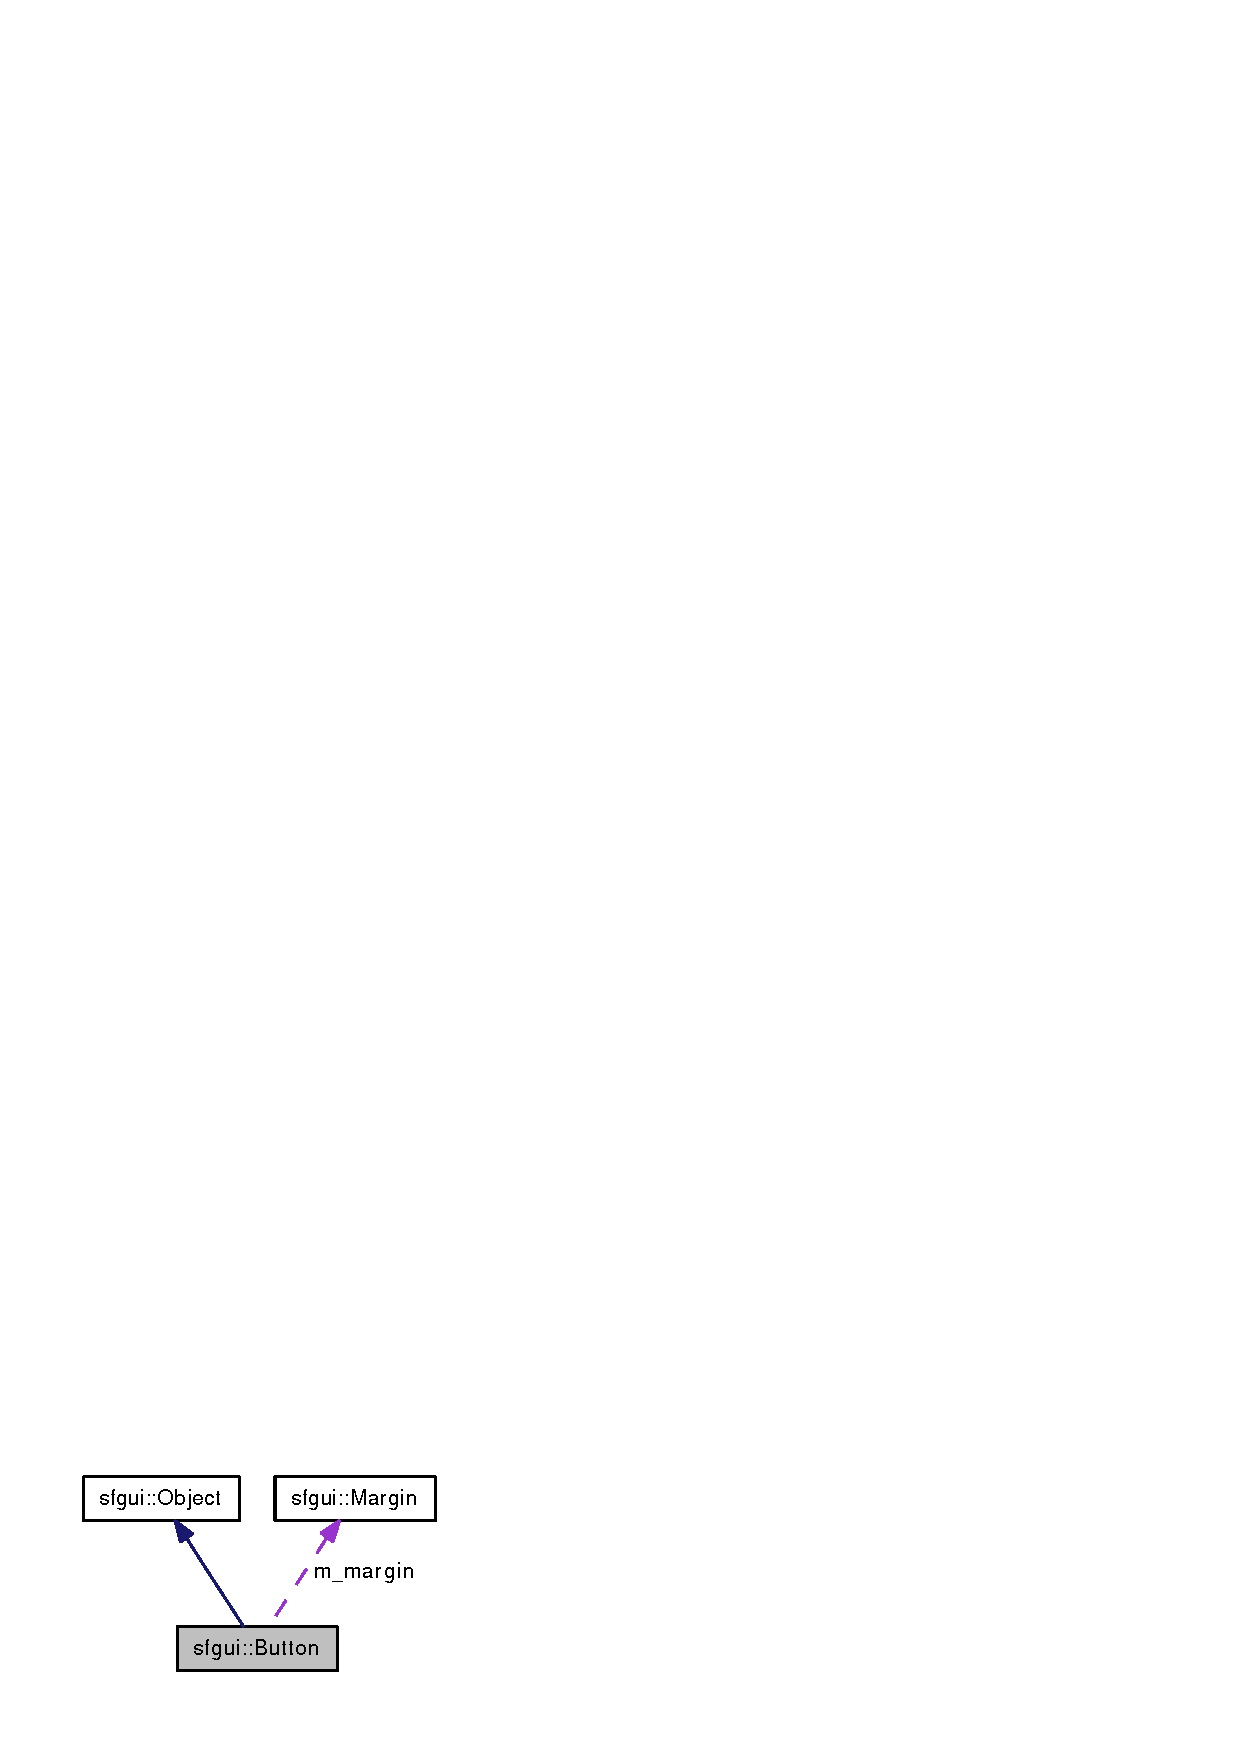
\includegraphics[width=106pt]{classsfgui_1_1Button__coll__graph}
\end{center}
\end{figure}
\subsection*{Public Member Functions}
\begin{CompactItemize}
\item 
\hyperlink{classsfgui_1_1Button_05c78461b775a073bed1e218586defd7}{Button} (sf::RenderWindow $\ast$parentWindow)
\item 
\hyperlink{classsfgui_1_1Button_835b0cbc92ef98e4c884398e036d26ca}{$\sim$Button} ()
\item 
std::string \hyperlink{classsfgui_1_1Button_015166159ef486c5001c5b58e79abc2d}{getText} ()
\item 
void \hyperlink{classsfgui_1_1Button_48ddf97b9a9f77517f5bf70e93df2b80}{SetText} (std::string text)
\item 
std::string \hyperlink{classsfgui_1_1Button_f731f8fe61ce30a7e405d8d3a56c5f22}{GetText} ()
\item 
void \hyperlink{classsfgui_1_1Button_af73ff1983944ea0969bf5c7421725c5}{SetTextColor} (sf::Color \&)
\item 
sf::Color \hyperlink{classsfgui_1_1Button_7eca4b2322ce0785e64bd2932912b974}{GetTextColor} ()
\item 
void \hyperlink{classsfgui_1_1Button_eed26d1a50f825f24ef1f2a16ef0b425}{SetTextSize} (float)
\item 
float \hyperlink{classsfgui_1_1Button_ed3a5fc8690d92ee59483b5dd7de6dbf}{GetTextSize} ()
\item 
void \hyperlink{classsfgui_1_1Button_f1a92c908326f7bd9973da154854a8bd}{SetTextFont} (sf::Font \&)
\item 
sf::Font \hyperlink{classsfgui_1_1Button_8b3a0a7ac0482c039e11bb615a55e86b}{GetTextFont} ()
\item 
void \hyperlink{classsfgui_1_1Button_c1c0fe577ad7bfa1367ad406ae087bd1}{SetTextAlignment} (int)
\item 
void \hyperlink{classsfgui_1_1Button_af84ec76e02e12c55667b960d80cc90b}{SetTextMargin} (float)
\item 
void \hyperlink{classsfgui_1_1Button_94b8976462b04b1a0e63542dd49aa7c8}{SetTextLeftMargin} (float)
\item 
void \hyperlink{classsfgui_1_1Button_4a4b4c339d001a0578c5e70b01ef164b}{SetTextRightMargin} (float)
\item 
void \hyperlink{classsfgui_1_1Button_cd571ac750ad4f9f957da40fb1ae23d7}{SetTextTopMargin} (float)
\item 
void \hyperlink{classsfgui_1_1Button_18a553fdcfbcf42d7764d3e039a72708}{SetTextBottomMargin} (float)
\item 
void \hyperlink{classsfgui_1_1Button_4160a1abdec76e06db9b34b80f5fa12c}{SetPosition} (float x, float y)
\item 
void \hyperlink{classsfgui_1_1Button_be36461c2e85c67b6cc42f3a6cba0468}{Move} (float x, float y)
\item 
void \hyperlink{classsfgui_1_1Button_94dc6919349ff5ca9f334cce78afbe39}{Show} ()
\end{CompactItemize}
\subsection*{Protected Member Functions}
\begin{CompactItemize}
\item 
void \hyperlink{classsfgui_1_1Button_1e1eade317f3b603011067e4997b0725}{updateTextPos} ()
\end{CompactItemize}
\subsection*{Protected Attributes}
\begin{CompactItemize}
\item 
sf::String \hyperlink{classsfgui_1_1Button_5a436a029fef79723eed0b024b5a7693}{m\_\-text}
\item 
int \hyperlink{classsfgui_1_1Button_b1ca3893cbff9b09f42e16377c0073f9}{m\_\-textAlignment}
\item 
\hyperlink{structsfgui_1_1Margin}{sfgui::Margin} \hyperlink{classsfgui_1_1Button_20ee48b44f31ad5b5de11dc3b00103a7}{m\_\-margin}
\end{CompactItemize}


\subsection{Detailed Description}
A push button. 

This class represents a push button graphic item. It provides some signals (call some useful callbacks) like clicked, mouseOver... 

\subsection{Constructor \& Destructor Documentation}
\hypertarget{classsfgui_1_1Button_05c78461b775a073bed1e218586defd7}{
\index{sfgui::Button@{sfgui::Button}!Button@{Button}}
\index{Button@{Button}!sfgui::Button@{sfgui::Button}}
\subsubsection[Button]{\setlength{\rightskip}{0pt plus 5cm}sfgui::Button::Button (sf::RenderWindow $\ast$ {\em parentWindow})}}
\label{classsfgui_1_1Button_05c78461b775a073bed1e218586defd7}




Create a \hyperlink{classsfgui_1_1Button}{Button} on the parent window. \hypertarget{classsfgui_1_1Button_835b0cbc92ef98e4c884398e036d26ca}{
\index{sfgui::Button@{sfgui::Button}!$\sim$Button@{$\sim$Button}}
\index{$\sim$Button@{$\sim$Button}!sfgui::Button@{sfgui::Button}}
\subsubsection[$\sim$Button]{\setlength{\rightskip}{0pt plus 5cm}sfgui::Button::$\sim$Button ()}}
\label{classsfgui_1_1Button_835b0cbc92ef98e4c884398e036d26ca}




\subsection{Member Function Documentation}
\hypertarget{classsfgui_1_1Button_1e1eade317f3b603011067e4997b0725}{
\index{sfgui::Button@{sfgui::Button}!updateTextPos@{updateTextPos}}
\index{updateTextPos@{updateTextPos}!sfgui::Button@{sfgui::Button}}
\subsubsection[updateTextPos]{\setlength{\rightskip}{0pt plus 5cm}void sfgui::Button::updateTextPos ()\hspace{0.3cm}{\tt  \mbox{[}protected\mbox{]}}}}
\label{classsfgui_1_1Button_1e1eade317f3b603011067e4997b0725}




This function is called internally when the position of the button is changed, when text changed (...) to adapt the text position so that it stays to the right alignment \hypertarget{classsfgui_1_1Button_015166159ef486c5001c5b58e79abc2d}{
\index{sfgui::Button@{sfgui::Button}!getText@{getText}}
\index{getText@{getText}!sfgui::Button@{sfgui::Button}}
\subsubsection[getText]{\setlength{\rightskip}{0pt plus 5cm}std::string sfgui::Button::getText ()\hspace{0.3cm}{\tt  \mbox{[}inline\mbox{]}}}}
\label{classsfgui_1_1Button_015166159ef486c5001c5b58e79abc2d}




Get the button text \hypertarget{classsfgui_1_1Button_48ddf97b9a9f77517f5bf70e93df2b80}{
\index{sfgui::Button@{sfgui::Button}!SetText@{SetText}}
\index{SetText@{SetText}!sfgui::Button@{sfgui::Button}}
\subsubsection[SetText]{\setlength{\rightskip}{0pt plus 5cm}void sfgui::Button::SetText (std::string {\em text})}}
\label{classsfgui_1_1Button_48ddf97b9a9f77517f5bf70e93df2b80}




Set the button text. \hypertarget{classsfgui_1_1Button_f731f8fe61ce30a7e405d8d3a56c5f22}{
\index{sfgui::Button@{sfgui::Button}!GetText@{GetText}}
\index{GetText@{GetText}!sfgui::Button@{sfgui::Button}}
\subsubsection[GetText]{\setlength{\rightskip}{0pt plus 5cm}std::string sfgui::Button::GetText ()}}
\label{classsfgui_1_1Button_f731f8fe61ce30a7e405d8d3a56c5f22}


\hypertarget{classsfgui_1_1Button_af73ff1983944ea0969bf5c7421725c5}{
\index{sfgui::Button@{sfgui::Button}!SetTextColor@{SetTextColor}}
\index{SetTextColor@{SetTextColor}!sfgui::Button@{sfgui::Button}}
\subsubsection[SetTextColor]{\setlength{\rightskip}{0pt plus 5cm}void sfgui::Button::SetTextColor (sf::Color \& {\em color})}}
\label{classsfgui_1_1Button_af73ff1983944ea0969bf5c7421725c5}


\hypertarget{classsfgui_1_1Button_7eca4b2322ce0785e64bd2932912b974}{
\index{sfgui::Button@{sfgui::Button}!GetTextColor@{GetTextColor}}
\index{GetTextColor@{GetTextColor}!sfgui::Button@{sfgui::Button}}
\subsubsection[GetTextColor]{\setlength{\rightskip}{0pt plus 5cm}sf::Color sfgui::Button::GetTextColor ()}}
\label{classsfgui_1_1Button_7eca4b2322ce0785e64bd2932912b974}


\hypertarget{classsfgui_1_1Button_eed26d1a50f825f24ef1f2a16ef0b425}{
\index{sfgui::Button@{sfgui::Button}!SetTextSize@{SetTextSize}}
\index{SetTextSize@{SetTextSize}!sfgui::Button@{sfgui::Button}}
\subsubsection[SetTextSize]{\setlength{\rightskip}{0pt plus 5cm}void sfgui::Button::SetTextSize (float {\em size})}}
\label{classsfgui_1_1Button_eed26d1a50f825f24ef1f2a16ef0b425}




Set size of the text \hypertarget{classsfgui_1_1Button_ed3a5fc8690d92ee59483b5dd7de6dbf}{
\index{sfgui::Button@{sfgui::Button}!GetTextSize@{GetTextSize}}
\index{GetTextSize@{GetTextSize}!sfgui::Button@{sfgui::Button}}
\subsubsection[GetTextSize]{\setlength{\rightskip}{0pt plus 5cm}float sfgui::Button::GetTextSize ()}}
\label{classsfgui_1_1Button_ed3a5fc8690d92ee59483b5dd7de6dbf}


\hypertarget{classsfgui_1_1Button_f1a92c908326f7bd9973da154854a8bd}{
\index{sfgui::Button@{sfgui::Button}!SetTextFont@{SetTextFont}}
\index{SetTextFont@{SetTextFont}!sfgui::Button@{sfgui::Button}}
\subsubsection[SetTextFont]{\setlength{\rightskip}{0pt plus 5cm}void sfgui::Button::SetTextFont (sf::Font \& {\em font})}}
\label{classsfgui_1_1Button_f1a92c908326f7bd9973da154854a8bd}


\hypertarget{classsfgui_1_1Button_8b3a0a7ac0482c039e11bb615a55e86b}{
\index{sfgui::Button@{sfgui::Button}!GetTextFont@{GetTextFont}}
\index{GetTextFont@{GetTextFont}!sfgui::Button@{sfgui::Button}}
\subsubsection[GetTextFont]{\setlength{\rightskip}{0pt plus 5cm}sf::Font sfgui::Button::GetTextFont ()}}
\label{classsfgui_1_1Button_8b3a0a7ac0482c039e11bb615a55e86b}


\hypertarget{classsfgui_1_1Button_c1c0fe577ad7bfa1367ad406ae087bd1}{
\index{sfgui::Button@{sfgui::Button}!SetTextAlignment@{SetTextAlignment}}
\index{SetTextAlignment@{SetTextAlignment}!sfgui::Button@{sfgui::Button}}
\subsubsection[SetTextAlignment]{\setlength{\rightskip}{0pt plus 5cm}void sfgui::Button::SetTextAlignment (int {\em al})}}
\label{classsfgui_1_1Button_c1c0fe577ad7bfa1367ad406ae087bd1}




This set the position of the text on the button. You should use one of the following constant value sfgui::LEFT, sfgui::RIGHT, sfgui::CENTER \hypertarget{classsfgui_1_1Button_af84ec76e02e12c55667b960d80cc90b}{
\index{sfgui::Button@{sfgui::Button}!SetTextMargin@{SetTextMargin}}
\index{SetTextMargin@{SetTextMargin}!sfgui::Button@{sfgui::Button}}
\subsubsection[SetTextMargin]{\setlength{\rightskip}{0pt plus 5cm}void sfgui::Button::SetTextMargin (float {\em margin})}}
\label{classsfgui_1_1Button_af84ec76e02e12c55667b960d80cc90b}




Set the global margin. The text will be spaced from the button each border by a number of pixels. \hypertarget{classsfgui_1_1Button_94b8976462b04b1a0e63542dd49aa7c8}{
\index{sfgui::Button@{sfgui::Button}!SetTextLeftMargin@{SetTextLeftMargin}}
\index{SetTextLeftMargin@{SetTextLeftMargin}!sfgui::Button@{sfgui::Button}}
\subsubsection[SetTextLeftMargin]{\setlength{\rightskip}{0pt plus 5cm}void sfgui::Button::SetTextLeftMargin (float {\em margin})}}
\label{classsfgui_1_1Button_94b8976462b04b1a0e63542dd49aa7c8}




Set the left margin. Text will be spaced from the left border of the button \hypertarget{classsfgui_1_1Button_4a4b4c339d001a0578c5e70b01ef164b}{
\index{sfgui::Button@{sfgui::Button}!SetTextRightMargin@{SetTextRightMargin}}
\index{SetTextRightMargin@{SetTextRightMargin}!sfgui::Button@{sfgui::Button}}
\subsubsection[SetTextRightMargin]{\setlength{\rightskip}{0pt plus 5cm}void sfgui::Button::SetTextRightMargin (float {\em margin})}}
\label{classsfgui_1_1Button_4a4b4c339d001a0578c5e70b01ef164b}




Set the right margin. Text will be spaced form the right border of the button. \hypertarget{classsfgui_1_1Button_cd571ac750ad4f9f957da40fb1ae23d7}{
\index{sfgui::Button@{sfgui::Button}!SetTextTopMargin@{SetTextTopMargin}}
\index{SetTextTopMargin@{SetTextTopMargin}!sfgui::Button@{sfgui::Button}}
\subsubsection[SetTextTopMargin]{\setlength{\rightskip}{0pt plus 5cm}void sfgui::Button::SetTextTopMargin (float {\em margin})}}
\label{classsfgui_1_1Button_cd571ac750ad4f9f957da40fb1ae23d7}




Set the top margin. Text will be spaced from the top border of the button. \hypertarget{classsfgui_1_1Button_18a553fdcfbcf42d7764d3e039a72708}{
\index{sfgui::Button@{sfgui::Button}!SetTextBottomMargin@{SetTextBottomMargin}}
\index{SetTextBottomMargin@{SetTextBottomMargin}!sfgui::Button@{sfgui::Button}}
\subsubsection[SetTextBottomMargin]{\setlength{\rightskip}{0pt plus 5cm}void sfgui::Button::SetTextBottomMargin (float {\em margin})}}
\label{classsfgui_1_1Button_18a553fdcfbcf42d7764d3e039a72708}




set the bottom margin. Text will be spaced from the bottom border of the button \hypertarget{classsfgui_1_1Button_4160a1abdec76e06db9b34b80f5fa12c}{
\index{sfgui::Button@{sfgui::Button}!SetPosition@{SetPosition}}
\index{SetPosition@{SetPosition}!sfgui::Button@{sfgui::Button}}
\subsubsection[SetPosition]{\setlength{\rightskip}{0pt plus 5cm}void sfgui::Button::SetPosition (float {\em x}, \/  float {\em y})}}
\label{classsfgui_1_1Button_4160a1abdec76e06db9b34b80f5fa12c}




Set the button position. Adjust the text position to keep the text in the choosen position (center, left, right...) \hypertarget{classsfgui_1_1Button_be36461c2e85c67b6cc42f3a6cba0468}{
\index{sfgui::Button@{sfgui::Button}!Move@{Move}}
\index{Move@{Move}!sfgui::Button@{sfgui::Button}}
\subsubsection[Move]{\setlength{\rightskip}{0pt plus 5cm}void sfgui::Button::Move (float {\em x}, \/  float {\em y})}}
\label{classsfgui_1_1Button_be36461c2e85c67b6cc42f3a6cba0468}




Move the button and adjust the text position \hypertarget{classsfgui_1_1Button_94dc6919349ff5ca9f334cce78afbe39}{
\index{sfgui::Button@{sfgui::Button}!Show@{Show}}
\index{Show@{Show}!sfgui::Button@{sfgui::Button}}
\subsubsection[Show]{\setlength{\rightskip}{0pt plus 5cm}void sfgui::Button::Show ()}}
\label{classsfgui_1_1Button_94dc6919349ff5ca9f334cce78afbe39}




Display the button on the parent window 

Reimplemented in \hyperlink{classsfgui_1_1TextEdit_1ee03247816213b34caaff365b160de0}{sfgui::TextEdit}.

\subsection{Member Data Documentation}
\hypertarget{classsfgui_1_1Button_5a436a029fef79723eed0b024b5a7693}{
\index{sfgui::Button@{sfgui::Button}!m\_\-text@{m\_\-text}}
\index{m\_\-text@{m\_\-text}!sfgui::Button@{sfgui::Button}}
\subsubsection[m\_\-text]{\setlength{\rightskip}{0pt plus 5cm}sf::String {\bf sfgui::Button::m\_\-text}\hspace{0.3cm}{\tt  \mbox{[}protected\mbox{]}}}}
\label{classsfgui_1_1Button_5a436a029fef79723eed0b024b5a7693}


\hypertarget{classsfgui_1_1Button_b1ca3893cbff9b09f42e16377c0073f9}{
\index{sfgui::Button@{sfgui::Button}!m\_\-textAlignment@{m\_\-textAlignment}}
\index{m\_\-textAlignment@{m\_\-textAlignment}!sfgui::Button@{sfgui::Button}}
\subsubsection[m\_\-textAlignment]{\setlength{\rightskip}{0pt plus 5cm}int {\bf sfgui::Button::m\_\-textAlignment}\hspace{0.3cm}{\tt  \mbox{[}protected\mbox{]}}}}
\label{classsfgui_1_1Button_b1ca3893cbff9b09f42e16377c0073f9}


\hypertarget{classsfgui_1_1Button_20ee48b44f31ad5b5de11dc3b00103a7}{
\index{sfgui::Button@{sfgui::Button}!m\_\-margin@{m\_\-margin}}
\index{m\_\-margin@{m\_\-margin}!sfgui::Button@{sfgui::Button}}
\subsubsection[m\_\-margin]{\setlength{\rightskip}{0pt plus 5cm}{\bf sfgui::Margin} {\bf sfgui::Button::m\_\-margin}\hspace{0.3cm}{\tt  \mbox{[}protected\mbox{]}}}}
\label{classsfgui_1_1Button_20ee48b44f31ad5b5de11dc3b00103a7}




The documentation for this class was generated from the following files:\begin{CompactItemize}
\item 
\hyperlink{button_8hpp}{button.hpp}\item 
\hyperlink{button_8cpp}{button.cpp}\end{CompactItemize}

\hypertarget{classsfgui_1_1Error}{
\section{sfgui::Error Class Reference}
\label{classsfgui_1_1Error}\index{sfgui::Error@{sfgui::Error}}
}
{\tt \#include $<$error.hpp$>$}

\subsection*{Public Member Functions}
\begin{CompactItemize}
\item 
\hyperlink{classsfgui_1_1Error_d402c73e8bfc7b7883700ce2d6c0b7b1}{Error} (const char $\ast$phrase=\char`\"{}\char`\"{})  throw ()
\item 
virtual const char $\ast$ \hyperlink{classsfgui_1_1Error_7e169ba3f26b7585d292bec5a253b8ec}{what} () const   throw ()
\item 
virtual \hyperlink{classsfgui_1_1Error_fb2a732879909cf082f89002c0f03981}{$\sim$Error} ()  throw ()
\end{CompactItemize}
\subsection*{Private Attributes}
\begin{CompactItemize}
\item 
char const $\ast$ \hyperlink{classsfgui_1_1Error_2acba2e2ab334cd94bf392f26f9207ff}{m\_\-phrase}
\begin{CompactList}\small\item\em Description of the error. \item\end{CompactList}\end{CompactItemize}


\subsection{Constructor \& Destructor Documentation}
\hypertarget{classsfgui_1_1Error_d402c73e8bfc7b7883700ce2d6c0b7b1}{
\index{sfgui::Error@{sfgui::Error}!Error@{Error}}
\index{Error@{Error}!sfgui::Error@{sfgui::Error}}
\subsubsection[Error]{\setlength{\rightskip}{0pt plus 5cm}sfgui::Error::Error (const char $\ast$ {\em phrase} = {\tt \char`\"{}\char`\"{}})  throw ()\hspace{0.3cm}{\tt  \mbox{[}inline\mbox{]}}}}
\label{classsfgui_1_1Error_d402c73e8bfc7b7883700ce2d6c0b7b1}


\hypertarget{classsfgui_1_1Error_fb2a732879909cf082f89002c0f03981}{
\index{sfgui::Error@{sfgui::Error}!$\sim$Error@{$\sim$Error}}
\index{$\sim$Error@{$\sim$Error}!sfgui::Error@{sfgui::Error}}
\subsubsection[$\sim$Error]{\setlength{\rightskip}{0pt plus 5cm}virtual sfgui::Error::$\sim$Error ()  throw ()\hspace{0.3cm}{\tt  \mbox{[}inline, virtual\mbox{]}}}}
\label{classsfgui_1_1Error_fb2a732879909cf082f89002c0f03981}




\subsection{Member Function Documentation}
\hypertarget{classsfgui_1_1Error_7e169ba3f26b7585d292bec5a253b8ec}{
\index{sfgui::Error@{sfgui::Error}!what@{what}}
\index{what@{what}!sfgui::Error@{sfgui::Error}}
\subsubsection[what]{\setlength{\rightskip}{0pt plus 5cm}virtual const char$\ast$ sfgui::Error::what () const  throw ()\hspace{0.3cm}{\tt  \mbox{[}inline, virtual\mbox{]}}}}
\label{classsfgui_1_1Error_7e169ba3f26b7585d292bec5a253b8ec}




\subsection{Member Data Documentation}
\hypertarget{classsfgui_1_1Error_2acba2e2ab334cd94bf392f26f9207ff}{
\index{sfgui::Error@{sfgui::Error}!m\_\-phrase@{m\_\-phrase}}
\index{m\_\-phrase@{m\_\-phrase}!sfgui::Error@{sfgui::Error}}
\subsubsection[m\_\-phrase]{\setlength{\rightskip}{0pt plus 5cm}char const$\ast$ {\bf sfgui::Error::m\_\-phrase}\hspace{0.3cm}{\tt  \mbox{[}private\mbox{]}}}}
\label{classsfgui_1_1Error_2acba2e2ab334cd94bf392f26f9207ff}


Description of the error. 



The documentation for this class was generated from the following file:\begin{CompactItemize}
\item 
\hyperlink{error_8hpp}{error.hpp}\end{CompactItemize}

\hypertarget{structsfgui_1_1Margin}{
\section{sfgui::Margin Struct Reference}
\label{structsfgui_1_1Margin}\index{sfgui::Margin@{sfgui::Margin}}
}
Struct which contains margin values.  


{\tt \#include $<$margin.hpp$>$}

\subsection*{Public Member Functions}
\begin{CompactItemize}
\item 
void \hyperlink{structsfgui_1_1Margin_6a505d8275fe7965b863d437dd54b195}{SetMargin} (float)
\end{CompactItemize}
\subsection*{Public Attributes}
\begin{CompactItemize}
\item 
float \hyperlink{structsfgui_1_1Margin_fb75f9e4550f4eb5d26c6af936f7e098}{Left}
\begin{CompactList}\small\item\em Left margin value. \item\end{CompactList}\item 
float \hyperlink{structsfgui_1_1Margin_fef8bae507f9cc00a42f442256062b66}{Right}
\begin{CompactList}\small\item\em Right margin value. \item\end{CompactList}\item 
float \hyperlink{structsfgui_1_1Margin_1ab360b58e3be2e8385f8e4225508ea4}{Top}
\begin{CompactList}\small\item\em Top margin value. \item\end{CompactList}\item 
float \hyperlink{structsfgui_1_1Margin_f9b744e36bb7d913b20959f7c9516fa6}{Bottom}
\begin{CompactList}\small\item\em Bottom margin value. \item\end{CompactList}\end{CompactItemize}


\subsection{Detailed Description}
Struct which contains margin values. 

This struc contains the pixel spacing from each border of an object. The function SetMargin is provided for convenience as it set all the margin with the same value. 

\subsection{Member Function Documentation}
\hypertarget{structsfgui_1_1Margin_6a505d8275fe7965b863d437dd54b195}{
\index{sfgui::Margin@{sfgui::Margin}!SetMargin@{SetMargin}}
\index{SetMargin@{SetMargin}!sfgui::Margin@{sfgui::Margin}}
\subsubsection[SetMargin]{\setlength{\rightskip}{0pt plus 5cm}void sfgui::Margin::SetMargin (float {\em margin})}}
\label{structsfgui_1_1Margin_6a505d8275fe7965b863d437dd54b195}




\subsection{Member Data Documentation}
\hypertarget{structsfgui_1_1Margin_fb75f9e4550f4eb5d26c6af936f7e098}{
\index{sfgui::Margin@{sfgui::Margin}!Left@{Left}}
\index{Left@{Left}!sfgui::Margin@{sfgui::Margin}}
\subsubsection[Left]{\setlength{\rightskip}{0pt plus 5cm}float {\bf sfgui::Margin::Left}}}
\label{structsfgui_1_1Margin_fb75f9e4550f4eb5d26c6af936f7e098}


Left margin value. 

\hypertarget{structsfgui_1_1Margin_fef8bae507f9cc00a42f442256062b66}{
\index{sfgui::Margin@{sfgui::Margin}!Right@{Right}}
\index{Right@{Right}!sfgui::Margin@{sfgui::Margin}}
\subsubsection[Right]{\setlength{\rightskip}{0pt plus 5cm}float {\bf sfgui::Margin::Right}}}
\label{structsfgui_1_1Margin_fef8bae507f9cc00a42f442256062b66}


Right margin value. 

\hypertarget{structsfgui_1_1Margin_1ab360b58e3be2e8385f8e4225508ea4}{
\index{sfgui::Margin@{sfgui::Margin}!Top@{Top}}
\index{Top@{Top}!sfgui::Margin@{sfgui::Margin}}
\subsubsection[Top]{\setlength{\rightskip}{0pt plus 5cm}float {\bf sfgui::Margin::Top}}}
\label{structsfgui_1_1Margin_1ab360b58e3be2e8385f8e4225508ea4}


Top margin value. 

\hypertarget{structsfgui_1_1Margin_f9b744e36bb7d913b20959f7c9516fa6}{
\index{sfgui::Margin@{sfgui::Margin}!Bottom@{Bottom}}
\index{Bottom@{Bottom}!sfgui::Margin@{sfgui::Margin}}
\subsubsection[Bottom]{\setlength{\rightskip}{0pt plus 5cm}float {\bf sfgui::Margin::Bottom}}}
\label{structsfgui_1_1Margin_f9b744e36bb7d913b20959f7c9516fa6}


Bottom margin value. 



The documentation for this struct was generated from the following files:\begin{CompactItemize}
\item 
\hyperlink{margin_8hpp}{margin.hpp}\item 
\hyperlink{margin_8cpp}{margin.cpp}\end{CompactItemize}

\hypertarget{classsfgui_1_1Object}{
\section{sfgui::Object Class Reference}
\label{classsfgui_1_1Object}\index{sfgui::Object@{sfgui::Object}}
}
A simple graphic item.  


{\tt \#include $<$object.hpp$>$}

Inheritance diagram for sfgui::Object:\nopagebreak
\begin{figure}[H]
\begin{center}
\leavevmode
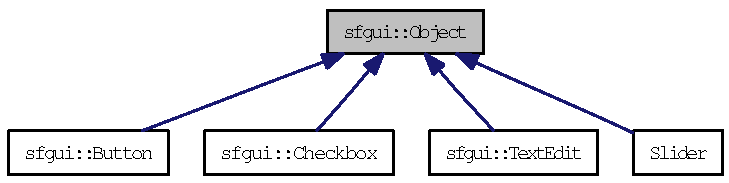
\includegraphics[width=400pt]{classsfgui_1_1Object__inherit__graph}
\end{center}
\end{figure}
Collaboration diagram for sfgui::Object:\nopagebreak
\begin{figure}[H]
\begin{center}
\leavevmode
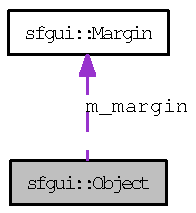
\includegraphics[width=65pt]{classsfgui_1_1Object__coll__graph}
\end{center}
\end{figure}
\subsection*{Public Member Functions}
\begin{CompactItemize}
\item 
\hyperlink{classsfgui_1_1Object_f03d0a10a3f8f71c58f56cf896e95f82}{Object} (sf::RenderWindow $\ast$parentWindow)
\item 
\hyperlink{classsfgui_1_1Object_6d0f96eda1f89ba15d34471cfa42a0e4}{Object} (sf::RenderWindow $\ast$parent, std::string themePath)
\item 
\hyperlink{classsfgui_1_1Object_7d923592a63a854c77ce4edcb21e40ba}{$\sim$Object} ()
\item 
void \hyperlink{classsfgui_1_1Object_96e00c4db6358d27ad806c0053e343a1}{SetTheme} (std::string)
\item 
void \hyperlink{classsfgui_1_1Object_b3477443fde0d86be5e32f5c1dcd7b01}{SetBackground} (int background)
\item 
void \hyperlink{classsfgui_1_1Object_64c05d85588778a652d11c7a1daf8db0}{SetText} (std::string text)
\item 
std::string \hyperlink{classsfgui_1_1Object_070ede7cda0e7b3cab312aac5013a206}{GetText} ()
\item 
void \hyperlink{classsfgui_1_1Object_88f1c97f50dd466417309f0776dce452}{SetTextColor} (sf::Color \&)
\item 
sf::Color \hyperlink{classsfgui_1_1Object_df734af2a7ca4ad600fe8bff51ed06cc}{GetTextColor} ()
\item 
void \hyperlink{classsfgui_1_1Object_6aba72276a557c90fef974478e88a04d}{SetTextSize} (int)
\item 
float \hyperlink{classsfgui_1_1Object_a6fae4cfa68982563c49b8b13b11966b}{GetTextSize} ()
\item 
void \hyperlink{classsfgui_1_1Object_41801231361e4866d99ce7d4ef32e53d}{SetTextFont} (sf::Font \&)
\item 
sf::Font \hyperlink{classsfgui_1_1Object_5f1d579d8ebba512fb983622552fe40f}{GetTextFont} ()
\item 
void \hyperlink{classsfgui_1_1Object_191bba44abbc751fd80e6f19ad6aba5b}{SetTextAlignment} (int)
\item 
void \hyperlink{classsfgui_1_1Object_f71c39eb2dfd2eb76e9be9e5dad606d9}{SetTextMargin} (float)
\item 
void \hyperlink{classsfgui_1_1Object_28408aa0cf50c8da37a79215755c01d9}{SetTextLeftMargin} (float)
\item 
void \hyperlink{classsfgui_1_1Object_dcea61673771a680fc47e4b838c2a59e}{SetTextRightMargin} (float)
\item 
void \hyperlink{classsfgui_1_1Object_6c3eb411a957d05707d858ded4cd951c}{SetTextTopMargin} (float)
\item 
void \hyperlink{classsfgui_1_1Object_db61eb19249fbbd28462cc79ca17b738}{SetTextBottomMargin} (float)
\item 
void \hyperlink{classsfgui_1_1Object_664c57bd35504a7d00963980d68dd022}{SetPosition} (float x, float y)
\item 
void \hyperlink{classsfgui_1_1Object_70b15fba99da515808d3da7d8042f458}{Move} (float x, float y)
\item 
void \hyperlink{classsfgui_1_1Object_cdf7f9b5f731e49e0e13e55de704805d}{Show} ()
\item 
void \hyperlink{classsfgui_1_1Object_c5d4f50f3d8712f098915cee5fc4ad41}{SetVisible} (bool)
\item 
void \hyperlink{classsfgui_1_1Object_e4711d5359ca3b756c9d4e063890cf16}{Hide} ()
\item 
void \hyperlink{classsfgui_1_1Object_cd9dbf2abe79e04c22f281bccb8bdb0e}{CheckEvent} (sf::Event Event)
\item 
void \hyperlink{classsfgui_1_1Object_d3d20a4cccde599748db724236ca0826}{SetClickCallback} (void($\ast$)())
\item 
void \hyperlink{classsfgui_1_1Object_8317dbdf44797dd69de490d4b946ed83}{SetMouseHoverCallback} (void($\ast$)())
\item 
void \hyperlink{classsfgui_1_1Object_3332575d988f9eee589f57b2ad516593}{ManageMouse} ()
\item 
void \hyperlink{classsfgui_1_1Object_da7f84701d318ce93fe59cc2f571eaf2}{Clicked} ()
\item 
void \hyperlink{classsfgui_1_1Object_68d1941ad05b3d0bdf2ba85702c04cc0}{MouseHover} ()
\item 
void \hyperlink{classsfgui_1_1Object_24575661efb4ab88be76eb2e1a4947e6}{MouseNotHover} ()
\end{CompactItemize}
\subsection*{Protected Types}
\begin{CompactItemize}
\item 
enum \hyperlink{classsfgui_1_1Object_8a7d7ae20a88b7ef8a104f7e6c8596ce}{ButtonStates} \{ \hyperlink{classsfgui_1_1Object_8a7d7ae20a88b7ef8a104f7e6c8596cee8211d79a1f35d08db2b31a914bddc38}{BackgroundNormal}, 
\hyperlink{classsfgui_1_1Object_8a7d7ae20a88b7ef8a104f7e6c8596ce03b529b6f0fee7ab7cc0033441180b67}{BackgroundClicked}, 
\hyperlink{classsfgui_1_1Object_8a7d7ae20a88b7ef8a104f7e6c8596ce9befc9dbae9107e3e7546af33a139df9}{BackgroundHover}
 \}
\end{CompactItemize}
\subsection*{Protected Member Functions}
\begin{CompactItemize}
\item 
void \hyperlink{classsfgui_1_1Object_27d9eb8b653f263f76b612cd77512321}{updateTextPos} ()
\end{CompactItemize}
\subsection*{Protected Attributes}
\begin{CompactItemize}
\item 
sf::String \hyperlink{classsfgui_1_1Object_b63c033215c2f6f1d64645e3c6f0153b}{m\_\-text}
\item 
std::string \hyperlink{classsfgui_1_1Object_d54c76d28fac3a92b8b97f1758a75685}{m\_\-tooltipTextStd}
\begin{CompactList}\small\item\em The std text for the tooltip message. \item\end{CompactList}\item 
sf::Font $\ast$ \hyperlink{classsfgui_1_1Object_20ec4624e3d9b8e3cebeb71ec97fd104}{m\_\-font}
\item 
int \hyperlink{classsfgui_1_1Object_7cfb56995f2140319df705fb1b146d36}{m\_\-textAlignment}
\item 
\hyperlink{structsfgui_1_1Margin}{sfgui::Margin} \hyperlink{classsfgui_1_1Object_b7afeee103f0cfc0c045effa8527a4b4}{m\_\-margin}
\item 
bool \hyperlink{classsfgui_1_1Object_105c5d17fb896da439156e5c198e5bb2}{m\_\-isVisible}
\item 
sf::RenderWindow $\ast$ \hyperlink{classsfgui_1_1Object_518ad23f1c9aab6fd9b346d708c503a8}{m\_\-parentRenderWindow}
\begin{CompactList}\small\item\em Pointer to the parent sf::RenderWindow. \item\end{CompactList}\item 
sf::Image $\ast$ \hyperlink{classsfgui_1_1Object_08225eee55352c02435d14e1bce24dbe}{m\_\-BackgroundImg}
\begin{CompactList}\small\item\em Curent background image. \item\end{CompactList}\item 
std::map$<$ int, sf::Image $\ast$ $>$ \hyperlink{classsfgui_1_1Object_6d7907f767742dcfd37c1b0c349daa2d}{m\_\-Images}
\item 
sf::Event \hyperlink{classsfgui_1_1Object_bd45c91f926c930806870ce8acbb955e}{m\_\-Event}
\begin{CompactList}\small\item\em Copy of the current sfml event. \item\end{CompactList}\end{CompactItemize}
\subsection*{Private Member Functions}
\begin{CompactItemize}
\item 
void \hyperlink{classsfgui_1_1Object_d2750b3d51a3a208739ed6c0c57df6aa}{generalInit} ()
\end{CompactItemize}
\subsection*{Private Attributes}
\begin{CompactItemize}
\item 
void($\ast$ \hyperlink{classsfgui_1_1Object_5917de9750aa3c8d282899ee83f835b4}{m\_\-clickCallback} )()
\begin{CompactList}\small\item\em Pointer to the click callback function. \item\end{CompactList}\item 
void($\ast$ \hyperlink{classsfgui_1_1Object_ddff61a2d47a7b25e05aa5b6311417ea}{m\_\-mouseHoverCallback} )()
\end{CompactItemize}


\subsection{Detailed Description}
A simple graphic item. 

This is a very simple object, which is rather useless (you can create a basic pushbutton, but not more). It's mostly present to be used as parent by other graphics items classes. This class create a sf::Sprite which represent a graphic item. There are some basic functions to set the general appearance like setBackground. This class can handle some common events which are possibly used by all widgets like clicks, mouse hover... 

\subsection{Member Enumeration Documentation}
\hypertarget{classsfgui_1_1Object_8a7d7ae20a88b7ef8a104f7e6c8596ce}{
\index{sfgui::Object@{sfgui::Object}!ButtonStates@{ButtonStates}}
\index{ButtonStates@{ButtonStates}!sfgui::Object@{sfgui::Object}}
\subsubsection[ButtonStates]{\setlength{\rightskip}{0pt plus 5cm}enum {\bf sfgui::Object::ButtonStates}\hspace{0.3cm}{\tt  \mbox{[}protected\mbox{]}}}}
\label{classsfgui_1_1Object_8a7d7ae20a88b7ef8a104f7e6c8596ce}


\begin{Desc}
\item[Enumerator: ]\par
\begin{description}
\index{BackgroundNormal@{BackgroundNormal}!sfgui::Object@{sfgui::Object}}\index{sfgui::Object@{sfgui::Object}!BackgroundNormal@{BackgroundNormal}}\item[{\em 
\hypertarget{classsfgui_1_1Object_8a7d7ae20a88b7ef8a104f7e6c8596cee8211d79a1f35d08db2b31a914bddc38}{
BackgroundNormal}
\label{classsfgui_1_1Object_8a7d7ae20a88b7ef8a104f7e6c8596cee8211d79a1f35d08db2b31a914bddc38}
}]\index{BackgroundClicked@{BackgroundClicked}!sfgui::Object@{sfgui::Object}}\index{sfgui::Object@{sfgui::Object}!BackgroundClicked@{BackgroundClicked}}\item[{\em 
\hypertarget{classsfgui_1_1Object_8a7d7ae20a88b7ef8a104f7e6c8596ce03b529b6f0fee7ab7cc0033441180b67}{
BackgroundClicked}
\label{classsfgui_1_1Object_8a7d7ae20a88b7ef8a104f7e6c8596ce03b529b6f0fee7ab7cc0033441180b67}
}]\index{BackgroundHover@{BackgroundHover}!sfgui::Object@{sfgui::Object}}\index{sfgui::Object@{sfgui::Object}!BackgroundHover@{BackgroundHover}}\item[{\em 
\hypertarget{classsfgui_1_1Object_8a7d7ae20a88b7ef8a104f7e6c8596ce9befc9dbae9107e3e7546af33a139df9}{
BackgroundHover}
\label{classsfgui_1_1Object_8a7d7ae20a88b7ef8a104f7e6c8596ce9befc9dbae9107e3e7546af33a139df9}
}]\end{description}
\end{Desc}



\subsection{Constructor \& Destructor Documentation}
\hypertarget{classsfgui_1_1Object_f03d0a10a3f8f71c58f56cf896e95f82}{
\index{sfgui::Object@{sfgui::Object}!Object@{Object}}
\index{Object@{Object}!sfgui::Object@{sfgui::Object}}
\subsubsection[Object]{\setlength{\rightskip}{0pt plus 5cm}sfgui::Object::Object (sf::RenderWindow $\ast$ {\em parentWindow})}}
\label{classsfgui_1_1Object_f03d0a10a3f8f71c58f56cf896e95f82}




Construct a simple graphic object

Load the default background images \hypertarget{classsfgui_1_1Object_6d0f96eda1f89ba15d34471cfa42a0e4}{
\index{sfgui::Object@{sfgui::Object}!Object@{Object}}
\index{Object@{Object}!sfgui::Object@{sfgui::Object}}
\subsubsection[Object]{\setlength{\rightskip}{0pt plus 5cm}sfgui::Object::Object (sf::RenderWindow $\ast$ {\em parent}, \/  std::string {\em themePath})}}
\label{classsfgui_1_1Object_6d0f96eda1f89ba15d34471cfa42a0e4}




Construct a graphic object which uses a custom theme instead of the default one. Instead of changing the theme by SetTheme, it's recomanded to use this constructor, as it directly loads the right images (it avoid loading images twices). \hypertarget{classsfgui_1_1Object_7d923592a63a854c77ce4edcb21e40ba}{
\index{sfgui::Object@{sfgui::Object}!$\sim$Object@{$\sim$Object}}
\index{$\sim$Object@{$\sim$Object}!sfgui::Object@{sfgui::Object}}
\subsubsection[$\sim$Object]{\setlength{\rightskip}{0pt plus 5cm}sfgui::Object::$\sim$Object ()}}
\label{classsfgui_1_1Object_7d923592a63a854c77ce4edcb21e40ba}




Delete all the pointers, free the image map... 

\subsection{Member Function Documentation}
\hypertarget{classsfgui_1_1Object_96e00c4db6358d27ad806c0053e343a1}{
\index{sfgui::Object@{sfgui::Object}!SetTheme@{SetTheme}}
\index{SetTheme@{SetTheme}!sfgui::Object@{sfgui::Object}}
\subsubsection[SetTheme]{\setlength{\rightskip}{0pt plus 5cm}void sfgui::Object::SetTheme (std::string {\em dir})}}
\label{classsfgui_1_1Object_96e00c4db6358d27ad806c0053e343a1}




Load a background theme from a directory containing the right png images : \begin{itemize}
\item button.png is the normal background \item button\_\-clicked.png is the clicked background \item button\_\-hover.png is the background showed when mouse is above the button \end{itemize}
\hypertarget{classsfgui_1_1Object_b3477443fde0d86be5e32f5c1dcd7b01}{
\index{sfgui::Object@{sfgui::Object}!SetBackground@{SetBackground}}
\index{SetBackground@{SetBackground}!sfgui::Object@{sfgui::Object}}
\subsubsection[SetBackground]{\setlength{\rightskip}{0pt plus 5cm}void sfgui::Object::SetBackground (int {\em background})}}
\label{classsfgui_1_1Object_b3477443fde0d86be5e32f5c1dcd7b01}




Set a background from an image which is already loaded int this object. {\bf Throws : }when an error occurs, like image index doesn't exists, it throw a \hyperlink{classsfgui_1_1Error}{sfgui::Error} \begin{Desc}
\item[Parameters:]
\begin{description}
\item[{\em background}]It is the num of the background. It must one of the followings values : \hyperlink{classsfgui_1_1Object_8a7d7ae20a88b7ef8a104f7e6c8596cee8211d79a1f35d08db2b31a914bddc38}{Object::BackgroundNormal}, \hyperlink{classsfgui_1_1Object_8a7d7ae20a88b7ef8a104f7e6c8596ce03b529b6f0fee7ab7cc0033441180b67}{Object::BackgroundClicked}, \hyperlink{classsfgui_1_1Object_8a7d7ae20a88b7ef8a104f7e6c8596ce9befc9dbae9107e3e7546af33a139df9}{Object::BackgroundHover} ... \end{description}
\end{Desc}
\begin{Desc}
\item[See also:]\hyperlink{classsfgui_1_1Object_8a7d7ae20a88b7ef8a104f7e6c8596ce}{sfgui::Object::ButtonStates} for the complete list of backgrounds values \end{Desc}
\hypertarget{classsfgui_1_1Object_64c05d85588778a652d11c7a1daf8db0}{
\index{sfgui::Object@{sfgui::Object}!SetText@{SetText}}
\index{SetText@{SetText}!sfgui::Object@{sfgui::Object}}
\subsubsection[SetText]{\setlength{\rightskip}{0pt plus 5cm}void sfgui::Object::SetText (std::string {\em text})}}
\label{classsfgui_1_1Object_64c05d85588778a652d11c7a1daf8db0}




Set the button text. 

Reimplemented in \hyperlink{classsfgui_1_1TextEdit_c6f06a7dc81611a50226e10287e87e1e}{sfgui::TextEdit}.\hypertarget{classsfgui_1_1Object_070ede7cda0e7b3cab312aac5013a206}{
\index{sfgui::Object@{sfgui::Object}!GetText@{GetText}}
\index{GetText@{GetText}!sfgui::Object@{sfgui::Object}}
\subsubsection[GetText]{\setlength{\rightskip}{0pt plus 5cm}std::string sfgui::Object::GetText ()}}
\label{classsfgui_1_1Object_070ede7cda0e7b3cab312aac5013a206}


\hypertarget{classsfgui_1_1Object_88f1c97f50dd466417309f0776dce452}{
\index{sfgui::Object@{sfgui::Object}!SetTextColor@{SetTextColor}}
\index{SetTextColor@{SetTextColor}!sfgui::Object@{sfgui::Object}}
\subsubsection[SetTextColor]{\setlength{\rightskip}{0pt plus 5cm}void sfgui::Object::SetTextColor (sf::Color \& {\em color})}}
\label{classsfgui_1_1Object_88f1c97f50dd466417309f0776dce452}


\hypertarget{classsfgui_1_1Object_df734af2a7ca4ad600fe8bff51ed06cc}{
\index{sfgui::Object@{sfgui::Object}!GetTextColor@{GetTextColor}}
\index{GetTextColor@{GetTextColor}!sfgui::Object@{sfgui::Object}}
\subsubsection[GetTextColor]{\setlength{\rightskip}{0pt plus 5cm}sf::Color sfgui::Object::GetTextColor ()}}
\label{classsfgui_1_1Object_df734af2a7ca4ad600fe8bff51ed06cc}


\hypertarget{classsfgui_1_1Object_6aba72276a557c90fef974478e88a04d}{
\index{sfgui::Object@{sfgui::Object}!SetTextSize@{SetTextSize}}
\index{SetTextSize@{SetTextSize}!sfgui::Object@{sfgui::Object}}
\subsubsection[SetTextSize]{\setlength{\rightskip}{0pt plus 5cm}void sfgui::Object::SetTextSize (int {\em size})}}
\label{classsfgui_1_1Object_6aba72276a557c90fef974478e88a04d}




Set size of the text \hypertarget{classsfgui_1_1Object_a6fae4cfa68982563c49b8b13b11966b}{
\index{sfgui::Object@{sfgui::Object}!GetTextSize@{GetTextSize}}
\index{GetTextSize@{GetTextSize}!sfgui::Object@{sfgui::Object}}
\subsubsection[GetTextSize]{\setlength{\rightskip}{0pt plus 5cm}float sfgui::Object::GetTextSize ()}}
\label{classsfgui_1_1Object_a6fae4cfa68982563c49b8b13b11966b}


\hypertarget{classsfgui_1_1Object_41801231361e4866d99ce7d4ef32e53d}{
\index{sfgui::Object@{sfgui::Object}!SetTextFont@{SetTextFont}}
\index{SetTextFont@{SetTextFont}!sfgui::Object@{sfgui::Object}}
\subsubsection[SetTextFont]{\setlength{\rightskip}{0pt plus 5cm}void sfgui::Object::SetTextFont (sf::Font \& {\em font})}}
\label{classsfgui_1_1Object_41801231361e4866d99ce7d4ef32e53d}




Set the text font. {\bf Warning : } For some inherited widets (such as \hyperlink{classsfgui_1_1TextEdit}{TextEdit}) a non monospaced font will cause problems (like text getting out of the font...). It is because SFML doesn't provide function to get charachter width (so it is based on a constant one, wich is get from one character). \hypertarget{classsfgui_1_1Object_5f1d579d8ebba512fb983622552fe40f}{
\index{sfgui::Object@{sfgui::Object}!GetTextFont@{GetTextFont}}
\index{GetTextFont@{GetTextFont}!sfgui::Object@{sfgui::Object}}
\subsubsection[GetTextFont]{\setlength{\rightskip}{0pt plus 5cm}sf::Font sfgui::Object::GetTextFont ()}}
\label{classsfgui_1_1Object_5f1d579d8ebba512fb983622552fe40f}


\hypertarget{classsfgui_1_1Object_191bba44abbc751fd80e6f19ad6aba5b}{
\index{sfgui::Object@{sfgui::Object}!SetTextAlignment@{SetTextAlignment}}
\index{SetTextAlignment@{SetTextAlignment}!sfgui::Object@{sfgui::Object}}
\subsubsection[SetTextAlignment]{\setlength{\rightskip}{0pt plus 5cm}void sfgui::Object::SetTextAlignment (int {\em al})}}
\label{classsfgui_1_1Object_191bba44abbc751fd80e6f19ad6aba5b}




This set the position of the text on the button. You should use one of the following constant value sfgui::LEFT, sfgui::RIGHT, sfgui::CENTER \hypertarget{classsfgui_1_1Object_f71c39eb2dfd2eb76e9be9e5dad606d9}{
\index{sfgui::Object@{sfgui::Object}!SetTextMargin@{SetTextMargin}}
\index{SetTextMargin@{SetTextMargin}!sfgui::Object@{sfgui::Object}}
\subsubsection[SetTextMargin]{\setlength{\rightskip}{0pt plus 5cm}void sfgui::Object::SetTextMargin (float {\em margin})}}
\label{classsfgui_1_1Object_f71c39eb2dfd2eb76e9be9e5dad606d9}




Set the global margin. The text will be spaced from the button each border by a number of pixels. \hypertarget{classsfgui_1_1Object_28408aa0cf50c8da37a79215755c01d9}{
\index{sfgui::Object@{sfgui::Object}!SetTextLeftMargin@{SetTextLeftMargin}}
\index{SetTextLeftMargin@{SetTextLeftMargin}!sfgui::Object@{sfgui::Object}}
\subsubsection[SetTextLeftMargin]{\setlength{\rightskip}{0pt plus 5cm}void sfgui::Object::SetTextLeftMargin (float {\em margin})}}
\label{classsfgui_1_1Object_28408aa0cf50c8da37a79215755c01d9}




Set the left margin. Text will be spaced from the left border of the button \hypertarget{classsfgui_1_1Object_dcea61673771a680fc47e4b838c2a59e}{
\index{sfgui::Object@{sfgui::Object}!SetTextRightMargin@{SetTextRightMargin}}
\index{SetTextRightMargin@{SetTextRightMargin}!sfgui::Object@{sfgui::Object}}
\subsubsection[SetTextRightMargin]{\setlength{\rightskip}{0pt plus 5cm}void sfgui::Object::SetTextRightMargin (float {\em margin})}}
\label{classsfgui_1_1Object_dcea61673771a680fc47e4b838c2a59e}




Set the right margin. Text will be spaced form the right border of the button. \hypertarget{classsfgui_1_1Object_6c3eb411a957d05707d858ded4cd951c}{
\index{sfgui::Object@{sfgui::Object}!SetTextTopMargin@{SetTextTopMargin}}
\index{SetTextTopMargin@{SetTextTopMargin}!sfgui::Object@{sfgui::Object}}
\subsubsection[SetTextTopMargin]{\setlength{\rightskip}{0pt plus 5cm}void sfgui::Object::SetTextTopMargin (float {\em margin})}}
\label{classsfgui_1_1Object_6c3eb411a957d05707d858ded4cd951c}




Set the top margin. Text will be spaced from the top border of the button. \hypertarget{classsfgui_1_1Object_db61eb19249fbbd28462cc79ca17b738}{
\index{sfgui::Object@{sfgui::Object}!SetTextBottomMargin@{SetTextBottomMargin}}
\index{SetTextBottomMargin@{SetTextBottomMargin}!sfgui::Object@{sfgui::Object}}
\subsubsection[SetTextBottomMargin]{\setlength{\rightskip}{0pt plus 5cm}void sfgui::Object::SetTextBottomMargin (float {\em margin})}}
\label{classsfgui_1_1Object_db61eb19249fbbd28462cc79ca17b738}




set the bottom margin. Text will be spaced from the bottom border of the button \hypertarget{classsfgui_1_1Object_664c57bd35504a7d00963980d68dd022}{
\index{sfgui::Object@{sfgui::Object}!SetPosition@{SetPosition}}
\index{SetPosition@{SetPosition}!sfgui::Object@{sfgui::Object}}
\subsubsection[SetPosition]{\setlength{\rightskip}{0pt plus 5cm}void sfgui::Object::SetPosition (float {\em x}, \/  float {\em y})}}
\label{classsfgui_1_1Object_664c57bd35504a7d00963980d68dd022}




Set the button position. Adjust the text position to keep the text in the choosen position (center, left, right...) \hypertarget{classsfgui_1_1Object_70b15fba99da515808d3da7d8042f458}{
\index{sfgui::Object@{sfgui::Object}!Move@{Move}}
\index{Move@{Move}!sfgui::Object@{sfgui::Object}}
\subsubsection[Move]{\setlength{\rightskip}{0pt plus 5cm}void sfgui::Object::Move (float {\em x}, \/  float {\em y})}}
\label{classsfgui_1_1Object_70b15fba99da515808d3da7d8042f458}




Move the button and adjust the text position \hypertarget{classsfgui_1_1Object_cdf7f9b5f731e49e0e13e55de704805d}{
\index{sfgui::Object@{sfgui::Object}!Show@{Show}}
\index{Show@{Show}!sfgui::Object@{sfgui::Object}}
\subsubsection[Show]{\setlength{\rightskip}{0pt plus 5cm}void sfgui::Object::Show ()}}
\label{classsfgui_1_1Object_cdf7f9b5f731e49e0e13e55de704805d}




Display the object on the parent window if the \hyperlink{classsfgui_1_1Object}{Object} is visible. \begin{Desc}
\item[See also:]\hyperlink{classsfgui_1_1Object_c5d4f50f3d8712f098915cee5fc4ad41}{SetVisible} \end{Desc}


Reimplemented in \hyperlink{classsfgui_1_1Checkbox_0028c58d4579845c1bdf3cae7ec9af5a}{sfgui::Checkbox}, and \hyperlink{classsfgui_1_1TextEdit_1ee03247816213b34caaff365b160de0}{sfgui::TextEdit}.\hypertarget{classsfgui_1_1Object_c5d4f50f3d8712f098915cee5fc4ad41}{
\index{sfgui::Object@{sfgui::Object}!SetVisible@{SetVisible}}
\index{SetVisible@{SetVisible}!sfgui::Object@{sfgui::Object}}
\subsubsection[SetVisible]{\setlength{\rightskip}{0pt plus 5cm}void sfgui::Object::SetVisible (bool {\em state})}}
\label{classsfgui_1_1Object_c5d4f50f3d8712f098915cee5fc4ad41}




Set the visibility of the \hyperlink{classsfgui_1_1Object}{Object} : true if visible, false if not \hypertarget{classsfgui_1_1Object_e4711d5359ca3b756c9d4e063890cf16}{
\index{sfgui::Object@{sfgui::Object}!Hide@{Hide}}
\index{Hide@{Hide}!sfgui::Object@{sfgui::Object}}
\subsubsection[Hide]{\setlength{\rightskip}{0pt plus 5cm}void sfgui::Object::Hide ()}}
\label{classsfgui_1_1Object_e4711d5359ca3b756c9d4e063890cf16}


\hypertarget{classsfgui_1_1Object_cd9dbf2abe79e04c22f281bccb8bdb0e}{
\index{sfgui::Object@{sfgui::Object}!CheckEvent@{CheckEvent}}
\index{CheckEvent@{CheckEvent}!sfgui::Object@{sfgui::Object}}
\subsubsection[CheckEvent]{\setlength{\rightskip}{0pt plus 5cm}void sfgui::Object::CheckEvent (sf::Event {\em Event})}}
\label{classsfgui_1_1Object_cd9dbf2abe79e04c22f281bccb8bdb0e}




Call the callbacks functions if needed on the given Event. 

Reimplemented in \hyperlink{classsfgui_1_1Checkbox_d618a9010bef60b8ea2f11f893320fb8}{sfgui::Checkbox}, \hyperlink{classSlider_29b1b660a47bd4c2e2baaedf02a072c3}{Slider}, and \hyperlink{classsfgui_1_1TextEdit_af6d4be3633d3eb8bcc7a1007e324da8}{sfgui::TextEdit}.\hypertarget{classsfgui_1_1Object_d3d20a4cccde599748db724236ca0826}{
\index{sfgui::Object@{sfgui::Object}!SetClickCallback@{SetClickCallback}}
\index{SetClickCallback@{SetClickCallback}!sfgui::Object@{sfgui::Object}}
\subsubsection[SetClickCallback]{\setlength{\rightskip}{0pt plus 5cm}void sfgui::Object::SetClickCallback (void($\ast$)() {\em clickCallBack})}}
\label{classsfgui_1_1Object_d3d20a4cccde599748db724236ca0826}




Set a pointer to the callback function called when the user click on this object \hypertarget{classsfgui_1_1Object_8317dbdf44797dd69de490d4b946ed83}{
\index{sfgui::Object@{sfgui::Object}!SetMouseHoverCallback@{SetMouseHoverCallback}}
\index{SetMouseHoverCallback@{SetMouseHoverCallback}!sfgui::Object@{sfgui::Object}}
\subsubsection[SetMouseHoverCallback]{\setlength{\rightskip}{0pt plus 5cm}void sfgui::Object::SetMouseHoverCallback (void($\ast$)() {\em mouseHoverCallback})}}
\label{classsfgui_1_1Object_8317dbdf44797dd69de490d4b946ed83}




Set a pointer to the callback function called when the mouse is hover the button. \hypertarget{classsfgui_1_1Object_3332575d988f9eee589f57b2ad516593}{
\index{sfgui::Object@{sfgui::Object}!ManageMouse@{ManageMouse}}
\index{ManageMouse@{ManageMouse}!sfgui::Object@{sfgui::Object}}
\subsubsection[ManageMouse]{\setlength{\rightskip}{0pt plus 5cm}void sfgui::Object::ManageMouse ()}}
\label{classsfgui_1_1Object_3332575d988f9eee589f57b2ad516593}




Manage the mouse events. 

Reimplemented in \hyperlink{classsfgui_1_1Checkbox_a49cffa3e2bef0e96105cd9a9103e294}{sfgui::Checkbox}.\hypertarget{classsfgui_1_1Object_da7f84701d318ce93fe59cc2f571eaf2}{
\index{sfgui::Object@{sfgui::Object}!Clicked@{Clicked}}
\index{Clicked@{Clicked}!sfgui::Object@{sfgui::Object}}
\subsubsection[Clicked]{\setlength{\rightskip}{0pt plus 5cm}void sfgui::Object::Clicked ()}}
\label{classsfgui_1_1Object_da7f84701d318ce93fe59cc2f571eaf2}




Call the click callback function. It's automatically called by checkEvent, but you can also call it yourself if needed. 

Reimplemented in \hyperlink{classsfgui_1_1Checkbox_9dc5f05d2f6d960d9fd50c77be3b7d6f}{sfgui::Checkbox}.\hypertarget{classsfgui_1_1Object_68d1941ad05b3d0bdf2ba85702c04cc0}{
\index{sfgui::Object@{sfgui::Object}!MouseHover@{MouseHover}}
\index{MouseHover@{MouseHover}!sfgui::Object@{sfgui::Object}}
\subsubsection[MouseHover]{\setlength{\rightskip}{0pt plus 5cm}void sfgui::Object::MouseHover ()}}
\label{classsfgui_1_1Object_68d1941ad05b3d0bdf2ba85702c04cc0}




Called when the mouse is above the button \hypertarget{classsfgui_1_1Object_24575661efb4ab88be76eb2e1a4947e6}{
\index{sfgui::Object@{sfgui::Object}!MouseNotHover@{MouseNotHover}}
\index{MouseNotHover@{MouseNotHover}!sfgui::Object@{sfgui::Object}}
\subsubsection[MouseNotHover]{\setlength{\rightskip}{0pt plus 5cm}void sfgui::Object::MouseNotHover ()}}
\label{classsfgui_1_1Object_24575661efb4ab88be76eb2e1a4947e6}




Called when the mouse is not above the button. It restores the default button theme \hypertarget{classsfgui_1_1Object_d2750b3d51a3a208739ed6c0c57df6aa}{
\index{sfgui::Object@{sfgui::Object}!generalInit@{generalInit}}
\index{generalInit@{generalInit}!sfgui::Object@{sfgui::Object}}
\subsubsection[generalInit]{\setlength{\rightskip}{0pt plus 5cm}void sfgui::Object::generalInit ()\hspace{0.3cm}{\tt  \mbox{[}private\mbox{]}}}}
\label{classsfgui_1_1Object_d2750b3d51a3a208739ed6c0c57df6aa}




Initialise the parts shared by all constructors 

Reimplemented in \hyperlink{classsfgui_1_1Button_59849e58ed4c46061d71f7172cab4e4e}{sfgui::Button}.\hypertarget{classsfgui_1_1Object_27d9eb8b653f263f76b612cd77512321}{
\index{sfgui::Object@{sfgui::Object}!updateTextPos@{updateTextPos}}
\index{updateTextPos@{updateTextPos}!sfgui::Object@{sfgui::Object}}
\subsubsection[updateTextPos]{\setlength{\rightskip}{0pt plus 5cm}void sfgui::Object::updateTextPos ()\hspace{0.3cm}{\tt  \mbox{[}protected\mbox{]}}}}
\label{classsfgui_1_1Object_27d9eb8b653f263f76b612cd77512321}




This function is called internally when the position of the button is changed, when text changed (...) to adapt the text position so that it stays to the right alignment 

\subsection{Member Data Documentation}
\hypertarget{classsfgui_1_1Object_5917de9750aa3c8d282899ee83f835b4}{
\index{sfgui::Object@{sfgui::Object}!m\_\-clickCallback@{m\_\-clickCallback}}
\index{m\_\-clickCallback@{m\_\-clickCallback}!sfgui::Object@{sfgui::Object}}
\subsubsection[m\_\-clickCallback]{\setlength{\rightskip}{0pt plus 5cm}void($\ast$ {\bf sfgui::Object::m\_\-clickCallback})()\hspace{0.3cm}{\tt  \mbox{[}private\mbox{]}}}}
\label{classsfgui_1_1Object_5917de9750aa3c8d282899ee83f835b4}


Pointer to the click callback function. 

\hypertarget{classsfgui_1_1Object_ddff61a2d47a7b25e05aa5b6311417ea}{
\index{sfgui::Object@{sfgui::Object}!m\_\-mouseHoverCallback@{m\_\-mouseHoverCallback}}
\index{m\_\-mouseHoverCallback@{m\_\-mouseHoverCallback}!sfgui::Object@{sfgui::Object}}
\subsubsection[m\_\-mouseHoverCallback]{\setlength{\rightskip}{0pt plus 5cm}void($\ast$ {\bf sfgui::Object::m\_\-mouseHoverCallback})()\hspace{0.3cm}{\tt  \mbox{[}private\mbox{]}}}}
\label{classsfgui_1_1Object_ddff61a2d47a7b25e05aa5b6311417ea}


Pointer to the callback function called when mouse is hover the button \hypertarget{classsfgui_1_1Object_b63c033215c2f6f1d64645e3c6f0153b}{
\index{sfgui::Object@{sfgui::Object}!m\_\-text@{m\_\-text}}
\index{m\_\-text@{m\_\-text}!sfgui::Object@{sfgui::Object}}
\subsubsection[m\_\-text]{\setlength{\rightskip}{0pt plus 5cm}sf::String {\bf sfgui::Object::m\_\-text}\hspace{0.3cm}{\tt  \mbox{[}protected\mbox{]}}}}
\label{classsfgui_1_1Object_b63c033215c2f6f1d64645e3c6f0153b}


\hypertarget{classsfgui_1_1Object_d54c76d28fac3a92b8b97f1758a75685}{
\index{sfgui::Object@{sfgui::Object}!m\_\-tooltipTextStd@{m\_\-tooltipTextStd}}
\index{m\_\-tooltipTextStd@{m\_\-tooltipTextStd}!sfgui::Object@{sfgui::Object}}
\subsubsection[m\_\-tooltipTextStd]{\setlength{\rightskip}{0pt plus 5cm}std::string {\bf sfgui::Object::m\_\-tooltipTextStd}\hspace{0.3cm}{\tt  \mbox{[}protected\mbox{]}}}}
\label{classsfgui_1_1Object_d54c76d28fac3a92b8b97f1758a75685}


The std text for the tooltip message. 

\hypertarget{classsfgui_1_1Object_20ec4624e3d9b8e3cebeb71ec97fd104}{
\index{sfgui::Object@{sfgui::Object}!m\_\-font@{m\_\-font}}
\index{m\_\-font@{m\_\-font}!sfgui::Object@{sfgui::Object}}
\subsubsection[m\_\-font]{\setlength{\rightskip}{0pt plus 5cm}sf::Font$\ast$ {\bf sfgui::Object::m\_\-font}\hspace{0.3cm}{\tt  \mbox{[}protected\mbox{]}}}}
\label{classsfgui_1_1Object_20ec4624e3d9b8e3cebeb71ec97fd104}


\hypertarget{classsfgui_1_1Object_7cfb56995f2140319df705fb1b146d36}{
\index{sfgui::Object@{sfgui::Object}!m\_\-textAlignment@{m\_\-textAlignment}}
\index{m\_\-textAlignment@{m\_\-textAlignment}!sfgui::Object@{sfgui::Object}}
\subsubsection[m\_\-textAlignment]{\setlength{\rightskip}{0pt plus 5cm}int {\bf sfgui::Object::m\_\-textAlignment}\hspace{0.3cm}{\tt  \mbox{[}protected\mbox{]}}}}
\label{classsfgui_1_1Object_7cfb56995f2140319df705fb1b146d36}


\hypertarget{classsfgui_1_1Object_b7afeee103f0cfc0c045effa8527a4b4}{
\index{sfgui::Object@{sfgui::Object}!m\_\-margin@{m\_\-margin}}
\index{m\_\-margin@{m\_\-margin}!sfgui::Object@{sfgui::Object}}
\subsubsection[m\_\-margin]{\setlength{\rightskip}{0pt plus 5cm}{\bf sfgui::Margin} {\bf sfgui::Object::m\_\-margin}\hspace{0.3cm}{\tt  \mbox{[}protected\mbox{]}}}}
\label{classsfgui_1_1Object_b7afeee103f0cfc0c045effa8527a4b4}


\hypertarget{classsfgui_1_1Object_105c5d17fb896da439156e5c198e5bb2}{
\index{sfgui::Object@{sfgui::Object}!m\_\-isVisible@{m\_\-isVisible}}
\index{m\_\-isVisible@{m\_\-isVisible}!sfgui::Object@{sfgui::Object}}
\subsubsection[m\_\-isVisible]{\setlength{\rightskip}{0pt plus 5cm}bool {\bf sfgui::Object::m\_\-isVisible}\hspace{0.3cm}{\tt  \mbox{[}protected\mbox{]}}}}
\label{classsfgui_1_1Object_105c5d17fb896da439156e5c198e5bb2}


\hypertarget{classsfgui_1_1Object_518ad23f1c9aab6fd9b346d708c503a8}{
\index{sfgui::Object@{sfgui::Object}!m\_\-parentRenderWindow@{m\_\-parentRenderWindow}}
\index{m\_\-parentRenderWindow@{m\_\-parentRenderWindow}!sfgui::Object@{sfgui::Object}}
\subsubsection[m\_\-parentRenderWindow]{\setlength{\rightskip}{0pt plus 5cm}sf::RenderWindow$\ast$ {\bf sfgui::Object::m\_\-parentRenderWindow}\hspace{0.3cm}{\tt  \mbox{[}protected\mbox{]}}}}
\label{classsfgui_1_1Object_518ad23f1c9aab6fd9b346d708c503a8}


Pointer to the parent sf::RenderWindow. 

\hypertarget{classsfgui_1_1Object_08225eee55352c02435d14e1bce24dbe}{
\index{sfgui::Object@{sfgui::Object}!m\_\-BackgroundImg@{m\_\-BackgroundImg}}
\index{m\_\-BackgroundImg@{m\_\-BackgroundImg}!sfgui::Object@{sfgui::Object}}
\subsubsection[m\_\-BackgroundImg]{\setlength{\rightskip}{0pt plus 5cm}sf::Image$\ast$ {\bf sfgui::Object::m\_\-BackgroundImg}\hspace{0.3cm}{\tt  \mbox{[}protected\mbox{]}}}}
\label{classsfgui_1_1Object_08225eee55352c02435d14e1bce24dbe}


Curent background image. 

\hypertarget{classsfgui_1_1Object_6d7907f767742dcfd37c1b0c349daa2d}{
\index{sfgui::Object@{sfgui::Object}!m\_\-Images@{m\_\-Images}}
\index{m\_\-Images@{m\_\-Images}!sfgui::Object@{sfgui::Object}}
\subsubsection[m\_\-Images]{\setlength{\rightskip}{0pt plus 5cm}std::map$<$int, sf::Image $\ast$$>$ {\bf sfgui::Object::m\_\-Images}\hspace{0.3cm}{\tt  \mbox{[}protected\mbox{]}}}}
\label{classsfgui_1_1Object_6d7907f767742dcfd37c1b0c349daa2d}


\hypertarget{classsfgui_1_1Object_bd45c91f926c930806870ce8acbb955e}{
\index{sfgui::Object@{sfgui::Object}!m\_\-Event@{m\_\-Event}}
\index{m\_\-Event@{m\_\-Event}!sfgui::Object@{sfgui::Object}}
\subsubsection[m\_\-Event]{\setlength{\rightskip}{0pt plus 5cm}sf::Event {\bf sfgui::Object::m\_\-Event}\hspace{0.3cm}{\tt  \mbox{[}protected\mbox{]}}}}
\label{classsfgui_1_1Object_bd45c91f926c930806870ce8acbb955e}


Copy of the current sfml event. 



The documentation for this class was generated from the following files:\begin{CompactItemize}
\item 
/home/arnaud/programmation/sfml/sfgui/\hyperlink{object_8hpp}{object.hpp}\item 
/home/arnaud/programmation/sfml/sfgui/\hyperlink{object_8cpp}{object.cpp}\end{CompactItemize}

\hypertarget{classsfgui_1_1TextEdit}{
\section{sfgui::TextEdit Class Reference}
\label{classsfgui_1_1TextEdit}\index{sfgui::TextEdit@{sfgui::TextEdit}}
}
A single line text entry.  


{\tt \#include $<$textedit.hpp$>$}

Inheritance diagram for sfgui::TextEdit:\nopagebreak
\begin{figure}[H]
\begin{center}
\leavevmode
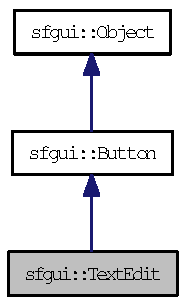
\includegraphics[width=62pt]{classsfgui_1_1TextEdit__inherit__graph}
\end{center}
\end{figure}
Collaboration diagram for sfgui::TextEdit:\nopagebreak
\begin{figure}[H]
\begin{center}
\leavevmode
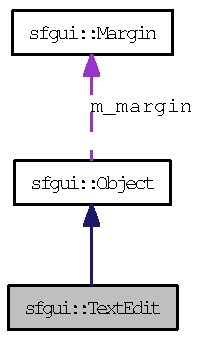
\includegraphics[width=106pt]{classsfgui_1_1TextEdit__coll__graph}
\end{center}
\end{figure}
\subsection*{Public Member Functions}
\begin{CompactItemize}
\item 
\hyperlink{classsfgui_1_1TextEdit_c6f2d938ccf876f05a9a9c47060c6093}{TextEdit} (sf::RenderWindow $\ast$parentWindow)
\item 
void \hyperlink{classsfgui_1_1TextEdit_16ffefa7f0c0d6e01275b8a2afa5975e}{SetText} (std::string \&)
\item 
void \hyperlink{classsfgui_1_1TextEdit_203952f38ce3bd68695597fee4b4397b}{AddChar} (char)
\item 
void \hyperlink{classsfgui_1_1TextEdit_dc95dab7bac1c41d0cebff1268f80c22}{DelChar} (int)
\item 
void \hyperlink{classsfgui_1_1TextEdit_bcd256e053ae8f13a5c7f919f79c03c9}{Activate} ()
\item 
void \hyperlink{classsfgui_1_1TextEdit_49b0919fd6c43c35913f8a46a6788270}{Deactivate} ()
\item 
void \hyperlink{classsfgui_1_1TextEdit_af6d4be3633d3eb8bcc7a1007e324da8}{CheckEvent} (sf::Event Event)
\item 
void \hyperlink{classsfgui_1_1TextEdit_2c80f417ea995a6452fcb47740701e1e}{SetTextChangedCallback} (void($\ast$)(std::string \&))
\item 
void \hyperlink{classsfgui_1_1TextEdit_b60f88cc667196bb073091e8878483f4}{SetReturnPressedCallback} (void($\ast$)())
\item 
void \hyperlink{classsfgui_1_1TextEdit_68bda298b3563eb960e77c3712664db8}{SetActivatedCallback} (void($\ast$)())
\item 
void \hyperlink{classsfgui_1_1TextEdit_6d75bcac8949d08513caa72e898e9b43}{SetDeactivatedCallback} (void($\ast$)())
\item 
void \hyperlink{classsfgui_1_1TextEdit_1ee03247816213b34caaff365b160de0}{Show} ()
\end{CompactItemize}
\subsection*{Private Member Functions}
\begin{CompactItemize}
\item 
void \hyperlink{classsfgui_1_1TextEdit_04bf790d96e0014479cc791691ecbade}{textChanged} ()
\item 
void \hyperlink{classsfgui_1_1TextEdit_c5ff761e3933294b46892db32e62b9f6}{deactivated} ()
\item 
void \hyperlink{classsfgui_1_1TextEdit_c009c601675801f2039d8f526e6fc921}{activated} ()
\end{CompactItemize}
\subsection*{Private Attributes}
\begin{CompactItemize}
\item 
std::string \hyperlink{classsfgui_1_1TextEdit_08de851a32aa8dd650e33dfcb376bfd8}{m\_\-stdText}
\item 
int \hyperlink{classsfgui_1_1TextEdit_648ee4daef549d909bef251aa2f12b40}{m\_\-nbCharToShow}
\item 
bool \hyperlink{classsfgui_1_1TextEdit_8ffa5546b2fd4901837b13a118f9beef}{m\_\-itemActive}
\item 
void($\ast$ \hyperlink{classsfgui_1_1TextEdit_a6d415ef1daf7f9fdf0dec3d71cb8eab}{m\_\-textChangedCallback} )(std::string \&)
\item 
void($\ast$ \hyperlink{classsfgui_1_1TextEdit_bfa97d7c95f54cc91600375242fe1ea6}{m\_\-deactivatedCallback} )()
\item 
void($\ast$ \hyperlink{classsfgui_1_1TextEdit_9cf910f9fca635f595d6a8963d7e30d1}{m\_\-activatedCallback} )()
\item 
void($\ast$ \hyperlink{classsfgui_1_1TextEdit_d86f9eaadf1313214631b2de009abf55}{m\_\-returnPressedCallback} )()
\end{CompactItemize}


\subsection{Detailed Description}
A single line text entry. 

This class provides a single line text entry widget. Thanks to this class, the user can enter text directly in the application, and usefull callbacks are provided, like textChangedCallback, returnPressedCallback.

\subsubsection*{Small tutorial}

If you want to enter text, you must have the item activated. You can activate it by calling the \hyperlink{classsfgui_1_1TextEdit_bcd256e053ae8f13a5c7f919f79c03c9}{Activate()} function (when user click on the \hyperlink{classsfgui_1_1TextEdit}{TextEdit}, this function is automatically called). \par
 If you want to stop typing text in the widget, you must call the \hyperlink{classsfgui_1_1TextEdit_49b0919fd6c43c35913f8a46a6788270}{Deactivate()} function. \par
 {\bf Important : you must call the CheckEvent function in the event loop. If you don't, the widget will just be shown, but won't work} 

\subsection{Constructor \& Destructor Documentation}
\hypertarget{classsfgui_1_1TextEdit_c6f2d938ccf876f05a9a9c47060c6093}{
\index{sfgui::TextEdit@{sfgui::TextEdit}!TextEdit@{TextEdit}}
\index{TextEdit@{TextEdit}!sfgui::TextEdit@{sfgui::TextEdit}}
\subsubsection[TextEdit]{\setlength{\rightskip}{0pt plus 5cm}sfgui::TextEdit::TextEdit (sf::RenderWindow $\ast$ {\em parentWindow})}}
\label{classsfgui_1_1TextEdit_c6f2d938ccf876f05a9a9c47060c6093}




\subsection{Member Function Documentation}
\hypertarget{classsfgui_1_1TextEdit_04bf790d96e0014479cc791691ecbade}{
\index{sfgui::TextEdit@{sfgui::TextEdit}!textChanged@{textChanged}}
\index{textChanged@{textChanged}!sfgui::TextEdit@{sfgui::TextEdit}}
\subsubsection[textChanged]{\setlength{\rightskip}{0pt plus 5cm}void sfgui::TextEdit::textChanged ()\hspace{0.3cm}{\tt  \mbox{[}private\mbox{]}}}}
\label{classsfgui_1_1TextEdit_04bf790d96e0014479cc791691ecbade}




If the text is modified, this function is called. It updates the sfString on the screen, and it call the textChanged callback (if exists) \hypertarget{classsfgui_1_1TextEdit_c5ff761e3933294b46892db32e62b9f6}{
\index{sfgui::TextEdit@{sfgui::TextEdit}!deactivated@{deactivated}}
\index{deactivated@{deactivated}!sfgui::TextEdit@{sfgui::TextEdit}}
\subsubsection[deactivated]{\setlength{\rightskip}{0pt plus 5cm}void sfgui::TextEdit::deactivated ()\hspace{0.3cm}{\tt  \mbox{[}private\mbox{]}}}}
\label{classsfgui_1_1TextEdit_c5ff761e3933294b46892db32e62b9f6}


\hypertarget{classsfgui_1_1TextEdit_c009c601675801f2039d8f526e6fc921}{
\index{sfgui::TextEdit@{sfgui::TextEdit}!activated@{activated}}
\index{activated@{activated}!sfgui::TextEdit@{sfgui::TextEdit}}
\subsubsection[activated]{\setlength{\rightskip}{0pt plus 5cm}void sfgui::TextEdit::activated ()\hspace{0.3cm}{\tt  \mbox{[}private\mbox{]}}}}
\label{classsfgui_1_1TextEdit_c009c601675801f2039d8f526e6fc921}


\hypertarget{classsfgui_1_1TextEdit_16ffefa7f0c0d6e01275b8a2afa5975e}{
\index{sfgui::TextEdit@{sfgui::TextEdit}!SetText@{SetText}}
\index{SetText@{SetText}!sfgui::TextEdit@{sfgui::TextEdit}}
\subsubsection[SetText]{\setlength{\rightskip}{0pt plus 5cm}void sfgui::TextEdit::SetText (std::string \& {\em text})}}
\label{classsfgui_1_1TextEdit_16ffefa7f0c0d6e01275b8a2afa5975e}




Set the text on the \hyperlink{classsfgui_1_1TextEdit}{TextEdit} \hypertarget{classsfgui_1_1TextEdit_203952f38ce3bd68695597fee4b4397b}{
\index{sfgui::TextEdit@{sfgui::TextEdit}!AddChar@{AddChar}}
\index{AddChar@{AddChar}!sfgui::TextEdit@{sfgui::TextEdit}}
\subsubsection[AddChar]{\setlength{\rightskip}{0pt plus 5cm}void sfgui::TextEdit::AddChar (char {\em ch})}}
\label{classsfgui_1_1TextEdit_203952f38ce3bd68695597fee4b4397b}




Add one char at the end of the current string \hypertarget{classsfgui_1_1TextEdit_dc95dab7bac1c41d0cebff1268f80c22}{
\index{sfgui::TextEdit@{sfgui::TextEdit}!DelChar@{DelChar}}
\index{DelChar@{DelChar}!sfgui::TextEdit@{sfgui::TextEdit}}
\subsubsection[DelChar]{\setlength{\rightskip}{0pt plus 5cm}void sfgui::TextEdit::DelChar (int {\em pos})}}
\label{classsfgui_1_1TextEdit_dc95dab7bac1c41d0cebff1268f80c22}




Delete one char from position pos \hypertarget{classsfgui_1_1TextEdit_bcd256e053ae8f13a5c7f919f79c03c9}{
\index{sfgui::TextEdit@{sfgui::TextEdit}!Activate@{Activate}}
\index{Activate@{Activate}!sfgui::TextEdit@{sfgui::TextEdit}}
\subsubsection[Activate]{\setlength{\rightskip}{0pt plus 5cm}void sfgui::TextEdit::Activate ()}}
\label{classsfgui_1_1TextEdit_bcd256e053ae8f13a5c7f919f79c03c9}




Activate the \hyperlink{classsfgui_1_1TextEdit}{TextEdit}. When the \hyperlink{classsfgui_1_1TextEdit}{TextEdit} is activated, all pressed keys are added to the \hyperlink{classsfgui_1_1TextEdit}{TextEdit} string \hypertarget{classsfgui_1_1TextEdit_49b0919fd6c43c35913f8a46a6788270}{
\index{sfgui::TextEdit@{sfgui::TextEdit}!Deactivate@{Deactivate}}
\index{Deactivate@{Deactivate}!sfgui::TextEdit@{sfgui::TextEdit}}
\subsubsection[Deactivate]{\setlength{\rightskip}{0pt plus 5cm}void sfgui::TextEdit::Deactivate ()}}
\label{classsfgui_1_1TextEdit_49b0919fd6c43c35913f8a46a6788270}




Deactivate the Textedit. Key you press will no longer be added to the \hyperlink{classsfgui_1_1TextEdit}{TextEdit} (until \hyperlink{classsfgui_1_1TextEdit_bcd256e053ae8f13a5c7f919f79c03c9}{Activate()} is called) \hypertarget{classsfgui_1_1TextEdit_af6d4be3633d3eb8bcc7a1007e324da8}{
\index{sfgui::TextEdit@{sfgui::TextEdit}!CheckEvent@{CheckEvent}}
\index{CheckEvent@{CheckEvent}!sfgui::TextEdit@{sfgui::TextEdit}}
\subsubsection[CheckEvent]{\setlength{\rightskip}{0pt plus 5cm}void sfgui::TextEdit::CheckEvent (sf::Event {\em Event})}}
\label{classsfgui_1_1TextEdit_af6d4be3633d3eb8bcc7a1007e324da8}


Callbacks 

Call the callbacks functions if needed on the given Event. 

Reimplemented from \hyperlink{classsfgui_1_1Object_cd9dbf2abe79e04c22f281bccb8bdb0e}{sfgui::Object}.\hypertarget{classsfgui_1_1TextEdit_2c80f417ea995a6452fcb47740701e1e}{
\index{sfgui::TextEdit@{sfgui::TextEdit}!SetTextChangedCallback@{SetTextChangedCallback}}
\index{SetTextChangedCallback@{SetTextChangedCallback}!sfgui::TextEdit@{sfgui::TextEdit}}
\subsubsection[SetTextChangedCallback]{\setlength{\rightskip}{0pt plus 5cm}void sfgui::TextEdit::SetTextChangedCallback (void($\ast$)(std::string \&) {\em textChangedCallback})}}
\label{classsfgui_1_1TextEdit_2c80f417ea995a6452fcb47740701e1e}




Set the callback called when the text is modified (add new char, delete one...) \hypertarget{classsfgui_1_1TextEdit_b60f88cc667196bb073091e8878483f4}{
\index{sfgui::TextEdit@{sfgui::TextEdit}!SetReturnPressedCallback@{SetReturnPressedCallback}}
\index{SetReturnPressedCallback@{SetReturnPressedCallback}!sfgui::TextEdit@{sfgui::TextEdit}}
\subsubsection[SetReturnPressedCallback]{\setlength{\rightskip}{0pt plus 5cm}void sfgui::TextEdit::SetReturnPressedCallback (void($\ast$)() {\em returnPressedCallback})}}
\label{classsfgui_1_1TextEdit_b60f88cc667196bb073091e8878483f4}




Set the callback called when the retun key is pressed (it can be used to know when the user finished his text entry for instance \hypertarget{classsfgui_1_1TextEdit_68bda298b3563eb960e77c3712664db8}{
\index{sfgui::TextEdit@{sfgui::TextEdit}!SetActivatedCallback@{SetActivatedCallback}}
\index{SetActivatedCallback@{SetActivatedCallback}!sfgui::TextEdit@{sfgui::TextEdit}}
\subsubsection[SetActivatedCallback]{\setlength{\rightskip}{0pt plus 5cm}void sfgui::TextEdit::SetActivatedCallback (void($\ast$)() {\em activatedCallback})}}
\label{classsfgui_1_1TextEdit_68bda298b3563eb960e77c3712664db8}




Set the callback called when the \hyperlink{classsfgui_1_1TextEdit}{TextEdit} is activated (ie has focus). \hypertarget{classsfgui_1_1TextEdit_6d75bcac8949d08513caa72e898e9b43}{
\index{sfgui::TextEdit@{sfgui::TextEdit}!SetDeactivatedCallback@{SetDeactivatedCallback}}
\index{SetDeactivatedCallback@{SetDeactivatedCallback}!sfgui::TextEdit@{sfgui::TextEdit}}
\subsubsection[SetDeactivatedCallback]{\setlength{\rightskip}{0pt plus 5cm}void sfgui::TextEdit::SetDeactivatedCallback (void($\ast$)() {\em deactivatedCallback})}}
\label{classsfgui_1_1TextEdit_6d75bcac8949d08513caa72e898e9b43}




Set the callback called when the \hyperlink{classsfgui_1_1TextEdit}{TextEdit} is deactivated (ie hasn't focus). \hypertarget{classsfgui_1_1TextEdit_1ee03247816213b34caaff365b160de0}{
\index{sfgui::TextEdit@{sfgui::TextEdit}!Show@{Show}}
\index{Show@{Show}!sfgui::TextEdit@{sfgui::TextEdit}}
\subsubsection[Show]{\setlength{\rightskip}{0pt plus 5cm}void sfgui::TextEdit::Show ()}}
\label{classsfgui_1_1TextEdit_1ee03247816213b34caaff365b160de0}




Show the \hyperlink{classsfgui_1_1TextEdit}{TextEdit} on the parent window 

Reimplemented from \hyperlink{classsfgui_1_1Button_94dc6919349ff5ca9f334cce78afbe39}{sfgui::Button}.

\subsection{Member Data Documentation}
\hypertarget{classsfgui_1_1TextEdit_08de851a32aa8dd650e33dfcb376bfd8}{
\index{sfgui::TextEdit@{sfgui::TextEdit}!m\_\-stdText@{m\_\-stdText}}
\index{m\_\-stdText@{m\_\-stdText}!sfgui::TextEdit@{sfgui::TextEdit}}
\subsubsection[m\_\-stdText]{\setlength{\rightskip}{0pt plus 5cm}std::string {\bf sfgui::TextEdit::m\_\-stdText}\hspace{0.3cm}{\tt  \mbox{[}private\mbox{]}}}}
\label{classsfgui_1_1TextEdit_08de851a32aa8dd650e33dfcb376bfd8}


\hypertarget{classsfgui_1_1TextEdit_648ee4daef549d909bef251aa2f12b40}{
\index{sfgui::TextEdit@{sfgui::TextEdit}!m\_\-nbCharToShow@{m\_\-nbCharToShow}}
\index{m\_\-nbCharToShow@{m\_\-nbCharToShow}!sfgui::TextEdit@{sfgui::TextEdit}}
\subsubsection[m\_\-nbCharToShow]{\setlength{\rightskip}{0pt plus 5cm}int {\bf sfgui::TextEdit::m\_\-nbCharToShow}\hspace{0.3cm}{\tt  \mbox{[}private\mbox{]}}}}
\label{classsfgui_1_1TextEdit_648ee4daef549d909bef251aa2f12b40}


\hypertarget{classsfgui_1_1TextEdit_8ffa5546b2fd4901837b13a118f9beef}{
\index{sfgui::TextEdit@{sfgui::TextEdit}!m\_\-itemActive@{m\_\-itemActive}}
\index{m\_\-itemActive@{m\_\-itemActive}!sfgui::TextEdit@{sfgui::TextEdit}}
\subsubsection[m\_\-itemActive]{\setlength{\rightskip}{0pt plus 5cm}bool {\bf sfgui::TextEdit::m\_\-itemActive}\hspace{0.3cm}{\tt  \mbox{[}private\mbox{]}}}}
\label{classsfgui_1_1TextEdit_8ffa5546b2fd4901837b13a118f9beef}


If true, user can enter text (textedit has focus), if false, it is disabled \hypertarget{classsfgui_1_1TextEdit_a6d415ef1daf7f9fdf0dec3d71cb8eab}{
\index{sfgui::TextEdit@{sfgui::TextEdit}!m\_\-textChangedCallback@{m\_\-textChangedCallback}}
\index{m\_\-textChangedCallback@{m\_\-textChangedCallback}!sfgui::TextEdit@{sfgui::TextEdit}}
\subsubsection[m\_\-textChangedCallback]{\setlength{\rightskip}{0pt plus 5cm}void($\ast$ {\bf sfgui::TextEdit::m\_\-textChangedCallback})(std::string \&)\hspace{0.3cm}{\tt  \mbox{[}private\mbox{]}}}}
\label{classsfgui_1_1TextEdit_a6d415ef1daf7f9fdf0dec3d71cb8eab}


\hypertarget{classsfgui_1_1TextEdit_bfa97d7c95f54cc91600375242fe1ea6}{
\index{sfgui::TextEdit@{sfgui::TextEdit}!m\_\-deactivatedCallback@{m\_\-deactivatedCallback}}
\index{m\_\-deactivatedCallback@{m\_\-deactivatedCallback}!sfgui::TextEdit@{sfgui::TextEdit}}
\subsubsection[m\_\-deactivatedCallback]{\setlength{\rightskip}{0pt plus 5cm}void($\ast$ {\bf sfgui::TextEdit::m\_\-deactivatedCallback})()\hspace{0.3cm}{\tt  \mbox{[}private\mbox{]}}}}
\label{classsfgui_1_1TextEdit_bfa97d7c95f54cc91600375242fe1ea6}


\hypertarget{classsfgui_1_1TextEdit_9cf910f9fca635f595d6a8963d7e30d1}{
\index{sfgui::TextEdit@{sfgui::TextEdit}!m\_\-activatedCallback@{m\_\-activatedCallback}}
\index{m\_\-activatedCallback@{m\_\-activatedCallback}!sfgui::TextEdit@{sfgui::TextEdit}}
\subsubsection[m\_\-activatedCallback]{\setlength{\rightskip}{0pt plus 5cm}void($\ast$ {\bf sfgui::TextEdit::m\_\-activatedCallback})()\hspace{0.3cm}{\tt  \mbox{[}private\mbox{]}}}}
\label{classsfgui_1_1TextEdit_9cf910f9fca635f595d6a8963d7e30d1}


\hypertarget{classsfgui_1_1TextEdit_d86f9eaadf1313214631b2de009abf55}{
\index{sfgui::TextEdit@{sfgui::TextEdit}!m\_\-returnPressedCallback@{m\_\-returnPressedCallback}}
\index{m\_\-returnPressedCallback@{m\_\-returnPressedCallback}!sfgui::TextEdit@{sfgui::TextEdit}}
\subsubsection[m\_\-returnPressedCallback]{\setlength{\rightskip}{0pt plus 5cm}void($\ast$ {\bf sfgui::TextEdit::m\_\-returnPressedCallback})()\hspace{0.3cm}{\tt  \mbox{[}private\mbox{]}}}}
\label{classsfgui_1_1TextEdit_d86f9eaadf1313214631b2de009abf55}




The documentation for this class was generated from the following files:\begin{CompactItemize}
\item 
\hyperlink{textedit_8hpp}{textedit.hpp}\item 
\hyperlink{textedit_8cpp}{textedit.cpp}\end{CompactItemize}

\chapter{File Documentation}
\hypertarget{button_8cpp}{
\section{/home/arnaud/programmation/sfml/sfgui/button.cpp File Reference}
\label{button_8cpp}\index{/home/arnaud/programmation/sfml/sfgui/button.cpp@{/home/arnaud/programmation/sfml/sfgui/button.cpp}}
}
{\tt \#include \char`\"{}button.hpp\char`\"{}}\par


Include dependency graph for button.cpp:\nopagebreak
\begin{figure}[H]
\begin{center}
\leavevmode
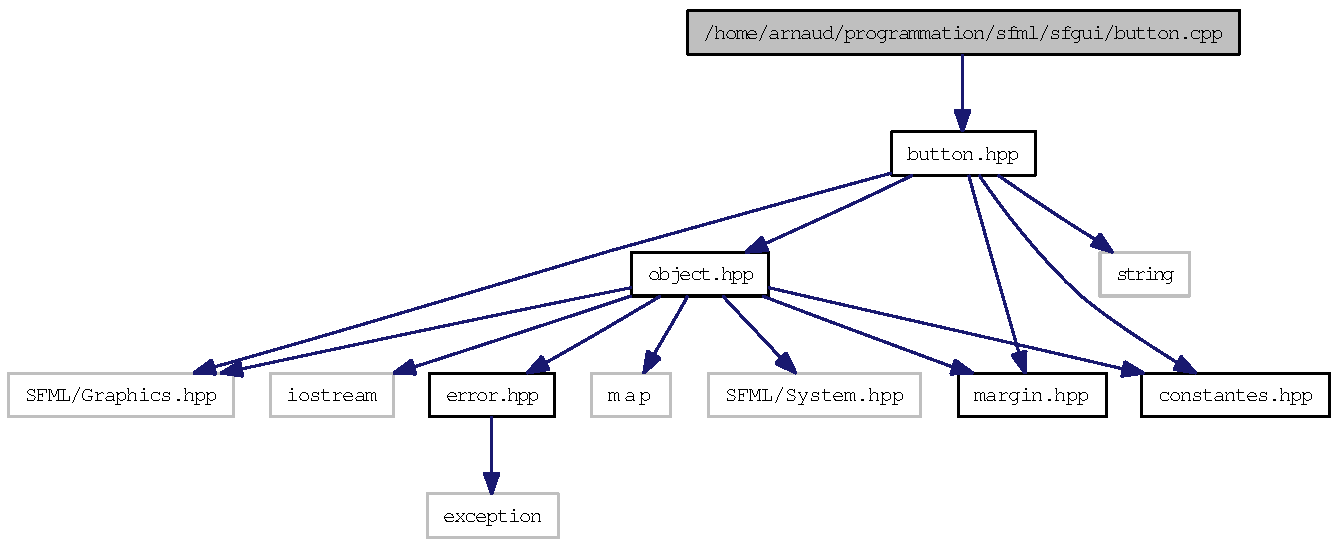
\includegraphics[width=279pt]{button_8cpp__incl}
\end{center}
\end{figure}

\hypertarget{button_8hpp}{
\section{/home/arnaud/programmation/sfml/sfgui/button.hpp File Reference}
\label{button_8hpp}\index{/home/arnaud/programmation/sfml/sfgui/button.hpp@{/home/arnaud/programmation/sfml/sfgui/button.hpp}}
}
{\tt \#include $<$SFML/Graphics.hpp$>$}\par
{\tt \#include \char`\"{}object.hpp\char`\"{}}\par
{\tt \#include \char`\"{}constantes.hpp\char`\"{}}\par
{\tt \#include \char`\"{}margin.hpp\char`\"{}}\par
{\tt \#include $<$string$>$}\par


Include dependency graph for button.hpp:\nopagebreak
\begin{figure}[H]
\begin{center}
\leavevmode
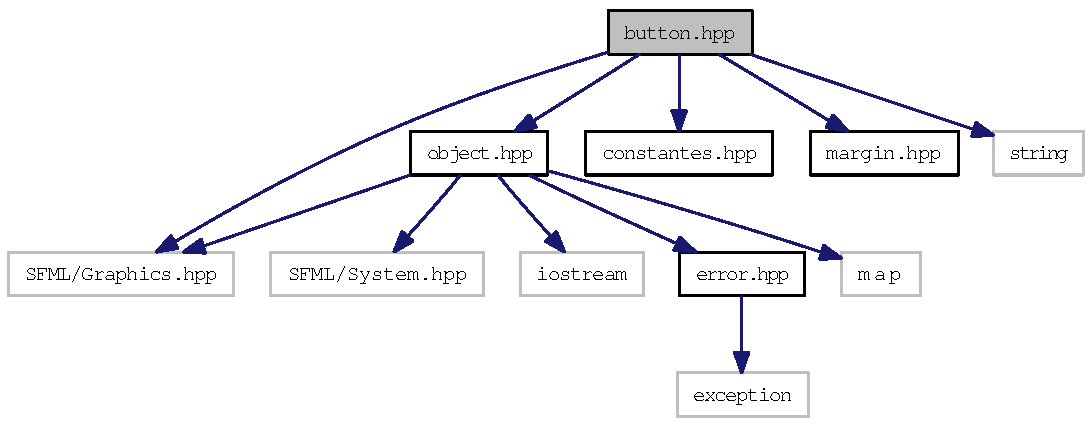
\includegraphics[width=279pt]{button_8hpp__incl}
\end{center}
\end{figure}


This graph shows which files directly or indirectly include this file:\nopagebreak
\begin{figure}[H]
\begin{center}
\leavevmode
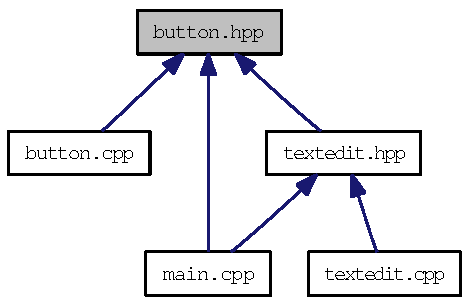
\includegraphics[width=376pt]{button_8hpp__dep__incl}
\end{center}
\end{figure}
\subsection*{Namespaces}
\begin{CompactItemize}
\item 
namespace \hyperlink{namespacesfgui}{sfgui}
\end{CompactItemize}
\subsection*{Classes}
\begin{CompactItemize}
\item 
class \hyperlink{classsfgui_1_1Button}{sfgui::Button}
\begin{CompactList}\small\item\em A push button. \item\end{CompactList}\end{CompactItemize}

\hypertarget{constantes_8hpp}{
\section{constantes.hpp File Reference}
\label{constantes_8hpp}\index{constantes.hpp@{constantes.hpp}}
}
Description not set. 



This graph shows which files directly or indirectly include this file:\nopagebreak
\begin{figure}[H]
\begin{center}
\leavevmode
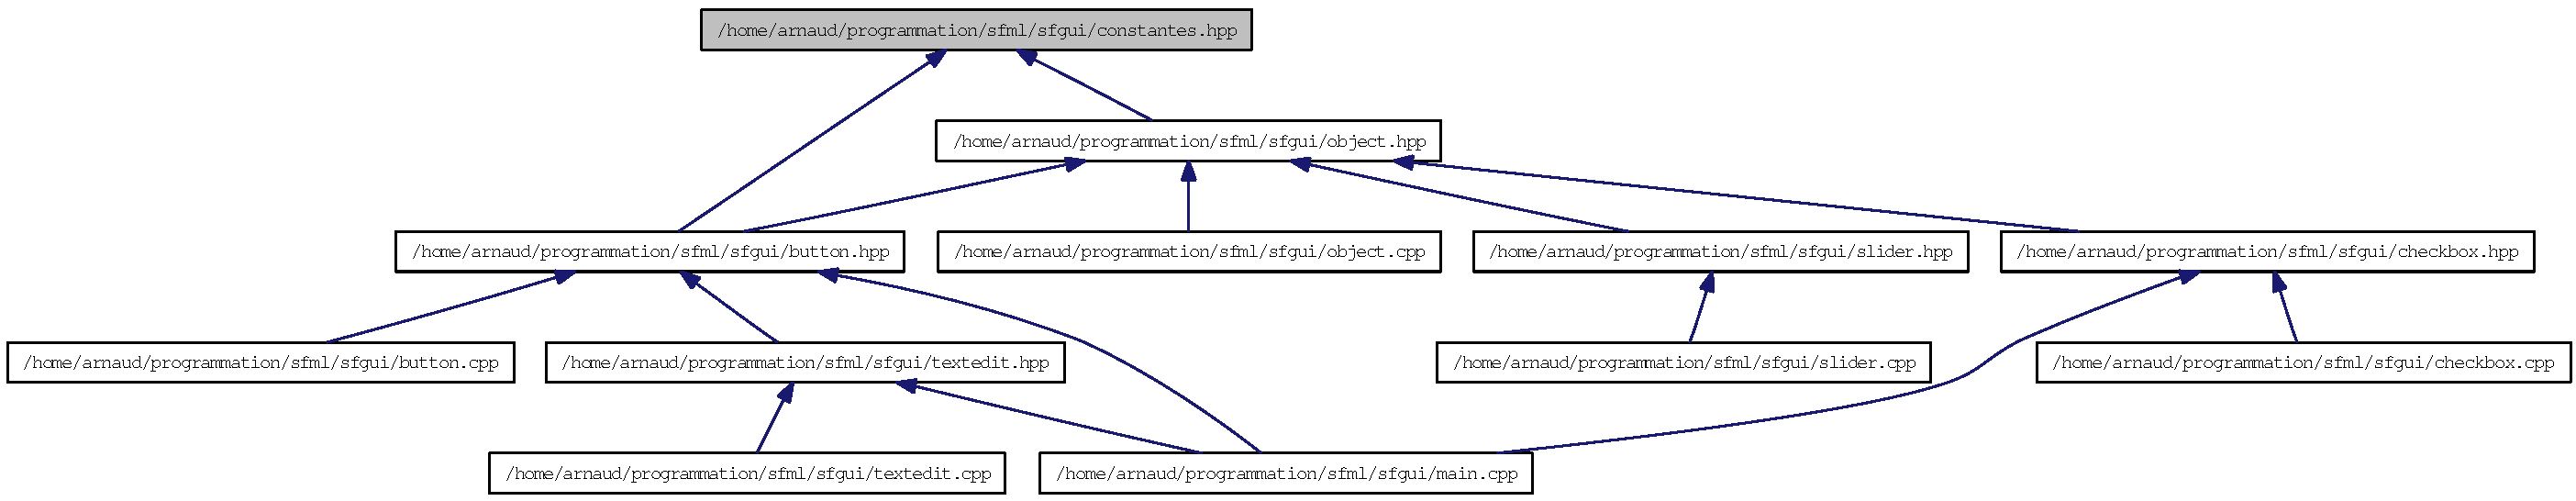
\includegraphics[width=130pt]{constantes_8hpp__dep__incl}
\end{center}
\end{figure}
\subsection*{Namespaces}
\begin{CompactItemize}
\item 
namespace \hyperlink{namespacesfgui}{sfgui}
\end{CompactItemize}
\subsection*{Enumerations}
\begin{CompactItemize}
\item 
enum \{ \hyperlink{namespacesfgui_ed969f0aaa542b462035e828757f431328ce9405120beac8fae51bc232aeabec}{sfgui::Left}, 
\hyperlink{namespacesfgui_ed969f0aaa542b462035e828757f4313d4fbbcf5a5a40412eeb0175f82c85b3f}{sfgui::Right}, 
\hyperlink{namespacesfgui_ed969f0aaa542b462035e828757f43130172869b534ad2378e28e388342699cc}{sfgui::Center}
 \}
\end{CompactItemize}


\subsection{Detailed Description}
Description not set. 

\begin{Desc}
\item[Author:]TANGUY Arnaud $<$\href{mailto:arn.tanguy@gmail.com}{\tt arn.tanguy@gmail.com}$>$ \end{Desc}
\begin{Desc}
\item[Date:]2009 \end{Desc}
\begin{Desc}
\item[Version:]0.1\end{Desc}
The big description for doxygen 
\hypertarget{error_8hpp}{
\section{/home/arnaud/programmation/sfml/sfgui/error.hpp File Reference}
\label{error_8hpp}\index{/home/arnaud/programmation/sfml/sfgui/error.hpp@{/home/arnaud/programmation/sfml/sfgui/error.hpp}}
}
{\tt \#include $<$exception$>$}\par


Include dependency graph for error.hpp:\nopagebreak
\begin{figure}[H]
\begin{center}
\leavevmode
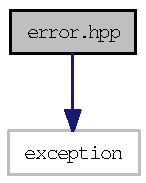
\includegraphics[width=150pt]{error_8hpp__incl}
\end{center}
\end{figure}


This graph shows which files directly or indirectly include this file:\nopagebreak
\begin{figure}[H]
\begin{center}
\leavevmode
\includegraphics[width=420pt]{error_8hpp__dep__incl}
\end{center}
\end{figure}
\subsection*{Namespaces}
\begin{CompactItemize}
\item 
namespace \hyperlink{namespacesfgui}{sfgui}
\end{CompactItemize}
\subsection*{Classes}
\begin{CompactItemize}
\item 
class \hyperlink{classsfgui_1_1Error}{sfgui::Error}
\end{CompactItemize}

\hypertarget{main_8cpp}{
\section{main.cpp File Reference}
\label{main_8cpp}\index{main.cpp@{main.cpp}}
}
{\tt \#include \char`\"{}button.hpp\char`\"{}}\par
{\tt \#include \char`\"{}textedit.hpp\char`\"{}}\par
{\tt \#include $<$iostream$>$}\par


Include dependency graph for main.cpp:\nopagebreak
\begin{figure}[H]
\begin{center}
\leavevmode
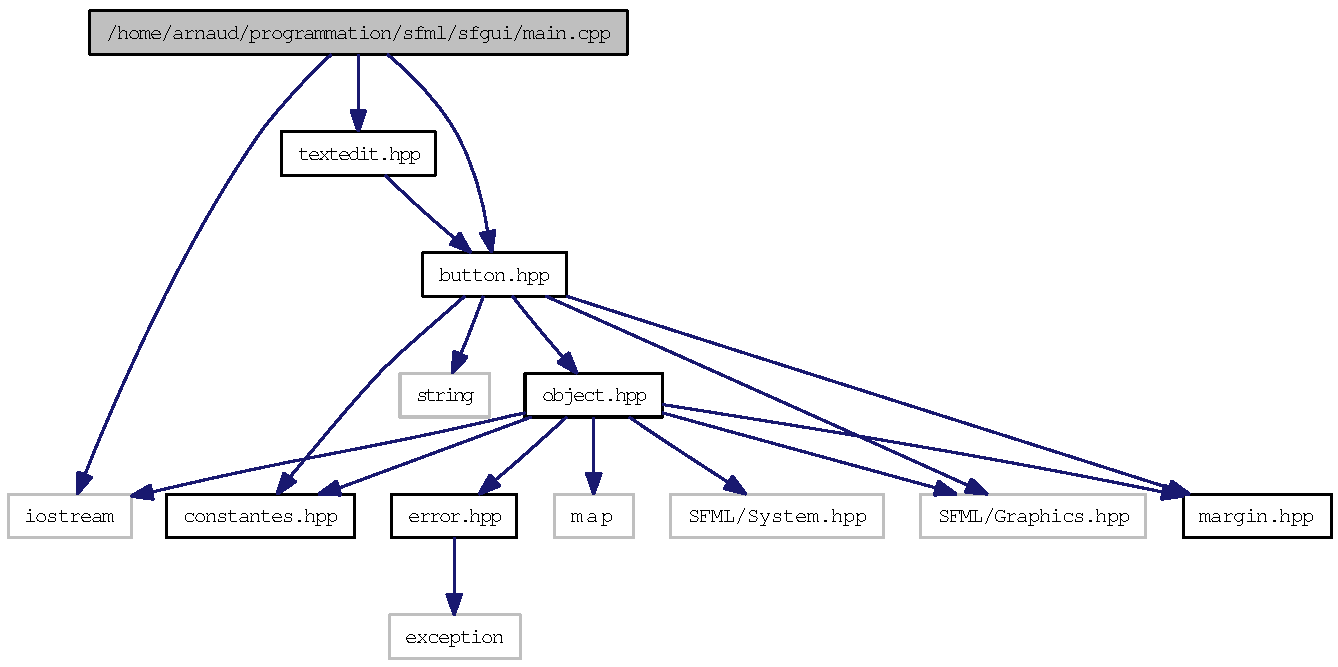
\includegraphics[width=262pt]{main_8cpp__incl}
\end{center}
\end{figure}
\subsection*{Functions}
\begin{CompactItemize}
\item 
sf::RenderWindow \hyperlink{main_8cpp_8991dd4eda96f401e33ee6ae24a46f0c}{App} (sf::VideoMode(800, 600, 32),\char`\"{}SFML GUI\char`\"{})
\item 
void \hyperlink{main_8cpp_fb33e4fdf2cfb177910c34fd0a19694d}{clickedCallBack} ()
\item 
void \hyperlink{main_8cpp_674037d7533f8891a97ed37d600aa1f9}{textChangeCallback} (std::string \&sr)
\item 
int \hyperlink{main_8cpp_e66f6b31b5ad750f1fe042a706a4e3d4}{main} ()
\end{CompactItemize}
\subsection*{Variables}
\begin{CompactItemize}
\item 
\hyperlink{classsfgui_1_1Button}{sfgui::Button} Sprite \& \hyperlink{main_8cpp_bcb2c6712035ac5e759315d67dced077}{App}
\end{CompactItemize}


\subsection{Function Documentation}
\hypertarget{main_8cpp_8991dd4eda96f401e33ee6ae24a46f0c}{
\index{main.cpp@{main.cpp}!App@{App}}
\index{App@{App}!main.cpp@{main.cpp}}
\subsubsection[App]{\setlength{\rightskip}{0pt plus 5cm}sf::RenderWindow App (sf:: {\em VideoMode}800, 600, 32, \/  \char`\"{}SFML GUI\char`\"{})}}
\label{main_8cpp_8991dd4eda96f401e33ee6ae24a46f0c}


\hypertarget{main_8cpp_fb33e4fdf2cfb177910c34fd0a19694d}{
\index{main.cpp@{main.cpp}!clickedCallBack@{clickedCallBack}}
\index{clickedCallBack@{clickedCallBack}!main.cpp@{main.cpp}}
\subsubsection[clickedCallBack]{\setlength{\rightskip}{0pt plus 5cm}void clickedCallBack ()}}
\label{main_8cpp_fb33e4fdf2cfb177910c34fd0a19694d}


\hypertarget{main_8cpp_e66f6b31b5ad750f1fe042a706a4e3d4}{
\index{main.cpp@{main.cpp}!main@{main}}
\index{main@{main}!main.cpp@{main.cpp}}
\subsubsection[main]{\setlength{\rightskip}{0pt plus 5cm}int main ()}}
\label{main_8cpp_e66f6b31b5ad750f1fe042a706a4e3d4}


\hypertarget{main_8cpp_674037d7533f8891a97ed37d600aa1f9}{
\index{main.cpp@{main.cpp}!textChangeCallback@{textChangeCallback}}
\index{textChangeCallback@{textChangeCallback}!main.cpp@{main.cpp}}
\subsubsection[textChangeCallback]{\setlength{\rightskip}{0pt plus 5cm}void textChangeCallback (std::string \& {\em sr})}}
\label{main_8cpp_674037d7533f8891a97ed37d600aa1f9}




\subsection{Variable Documentation}
\hypertarget{main_8cpp_bcb2c6712035ac5e759315d67dced077}{
\index{main.cpp@{main.cpp}!App@{App}}
\index{App@{App}!main.cpp@{main.cpp}}
\subsubsection[App]{\setlength{\rightskip}{0pt plus 5cm}{\bf sfgui::Button} Sprite\& App}}
\label{main_8cpp_bcb2c6712035ac5e759315d67dced077}



\hypertarget{margin_8cpp}{
\section{margin.cpp File Reference}
\label{margin_8cpp}\index{margin.cpp@{margin.cpp}}
}
{\tt \#include \char`\"{}margin.hpp\char`\"{}}\par


Include dependency graph for margin.cpp:\nopagebreak
\begin{figure}[H]
\begin{center}
\leavevmode
\includegraphics[width=57pt]{margin_8cpp__incl}
\end{center}
\end{figure}

\hypertarget{margin_8hpp}{
\section{/home/arnaud/programmation/sfml/sfgui/margin.hpp File Reference}
\label{margin_8hpp}\index{/home/arnaud/programmation/sfml/sfgui/margin.hpp@{/home/arnaud/programmation/sfml/sfgui/margin.hpp}}
}
A simple struct for margin. 



This graph shows which files directly or indirectly include this file:\nopagebreak
\begin{figure}[H]
\begin{center}
\leavevmode
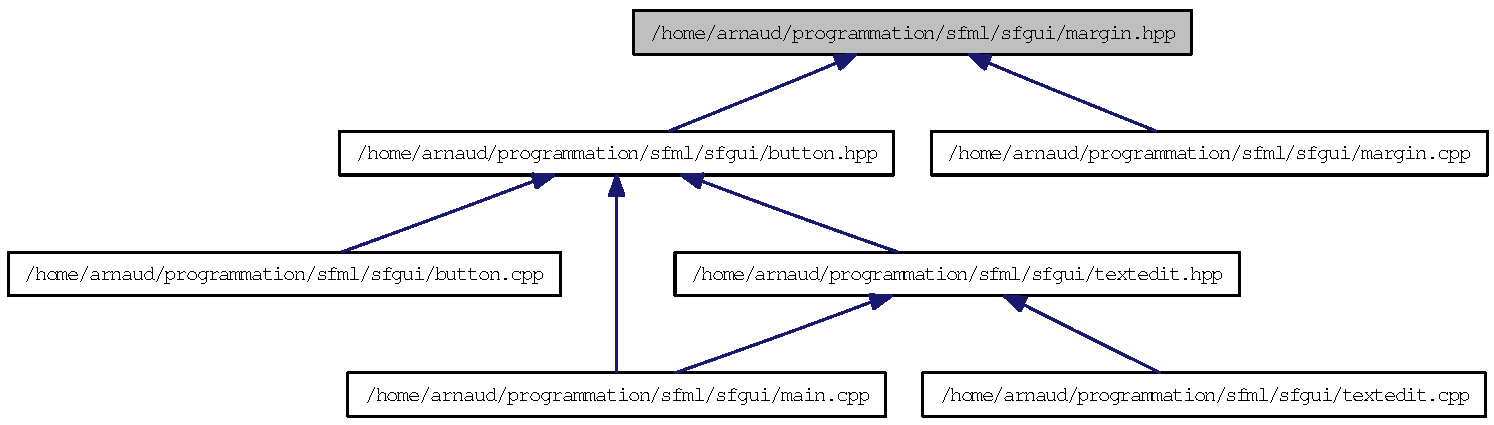
\includegraphics[width=420pt]{margin_8hpp__dep__incl}
\end{center}
\end{figure}
\subsection*{Namespaces}
\begin{CompactItemize}
\item 
namespace \hyperlink{namespacesfgui}{sfgui}
\end{CompactItemize}
\subsection*{Classes}
\begin{CompactItemize}
\item 
struct \hyperlink{structsfgui_1_1Margin}{sfgui::Margin}
\begin{CompactList}\small\item\em Struct which contains margin values. \item\end{CompactList}\end{CompactItemize}


\subsection{Detailed Description}
A simple struct for margin. 

\begin{Desc}
\item[Author:]TANGUY Arnaud $<$\href{mailto:arn.tanguy@gmail.com}{\tt arn.tanguy@gmail.com}$>$ \end{Desc}
\begin{Desc}
\item[Date:]2009 \end{Desc}
\begin{Desc}
\item[Version:]0.1 \end{Desc}

\hypertarget{object_8cpp}{
\section{/home/arnaud/programmation/sfml/sfgui/object.cpp File Reference}
\label{object_8cpp}\index{/home/arnaud/programmation/sfml/sfgui/object.cpp@{/home/arnaud/programmation/sfml/sfgui/object.cpp}}
}
{\tt \#include \char`\"{}object.hpp\char`\"{}}\par


Include dependency graph for object.cpp:\nopagebreak
\begin{figure}[H]
\begin{center}
\leavevmode
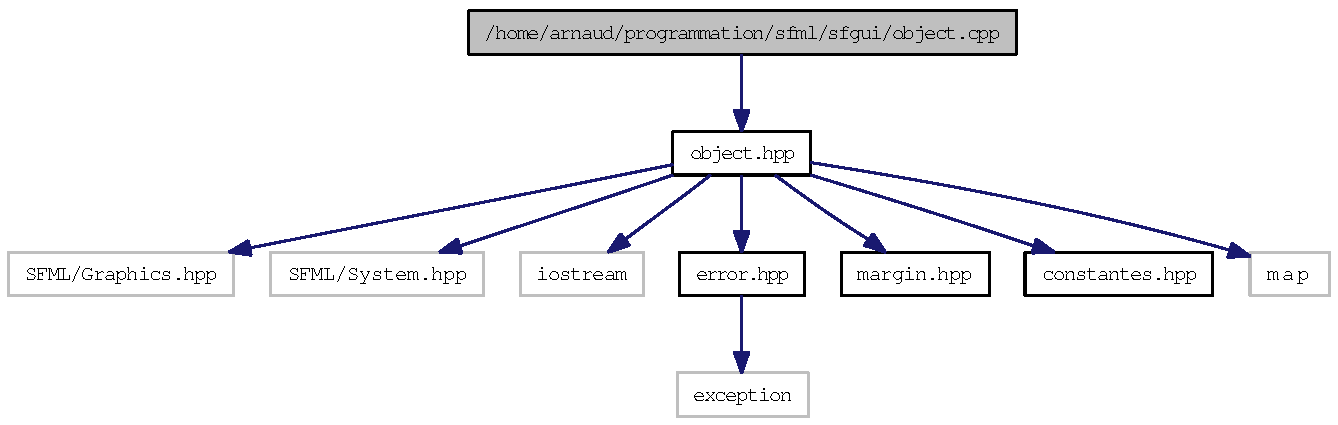
\includegraphics[width=241pt]{object_8cpp__incl}
\end{center}
\end{figure}

\hypertarget{object_8hpp}{
\section{/home/arnaud/programmation/sfml/sfgui/object.hpp File Reference}
\label{object_8hpp}\index{/home/arnaud/programmation/sfml/sfgui/object.hpp@{/home/arnaud/programmation/sfml/sfgui/object.hpp}}
}
{\tt \#include $<$SFML/Graphics.hpp$>$}\par
{\tt \#include $<$SFML/System.hpp$>$}\par
{\tt \#include $<$iostream$>$}\par
{\tt \#include \char`\"{}error.hpp\char`\"{}}\par
{\tt \#include \char`\"{}margin.hpp\char`\"{}}\par
{\tt \#include \char`\"{}constantes.hpp\char`\"{}}\par
{\tt \#include $<$map$>$}\par


Include dependency graph for object.hpp:\nopagebreak
\begin{figure}[H]
\begin{center}
\leavevmode
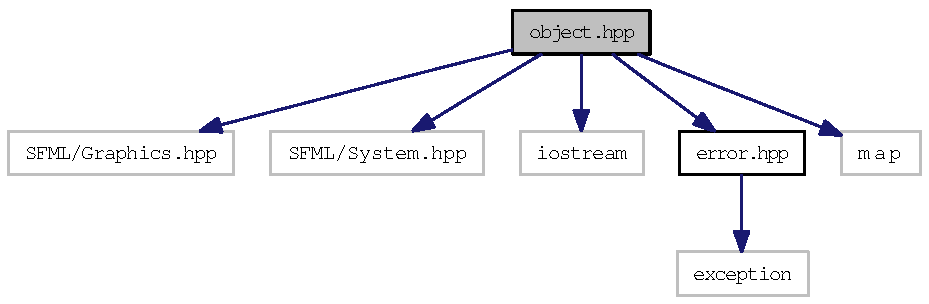
\includegraphics[width=339pt]{object_8hpp__incl}
\end{center}
\end{figure}


This graph shows which files directly or indirectly include this file:\nopagebreak
\begin{figure}[H]
\begin{center}
\leavevmode
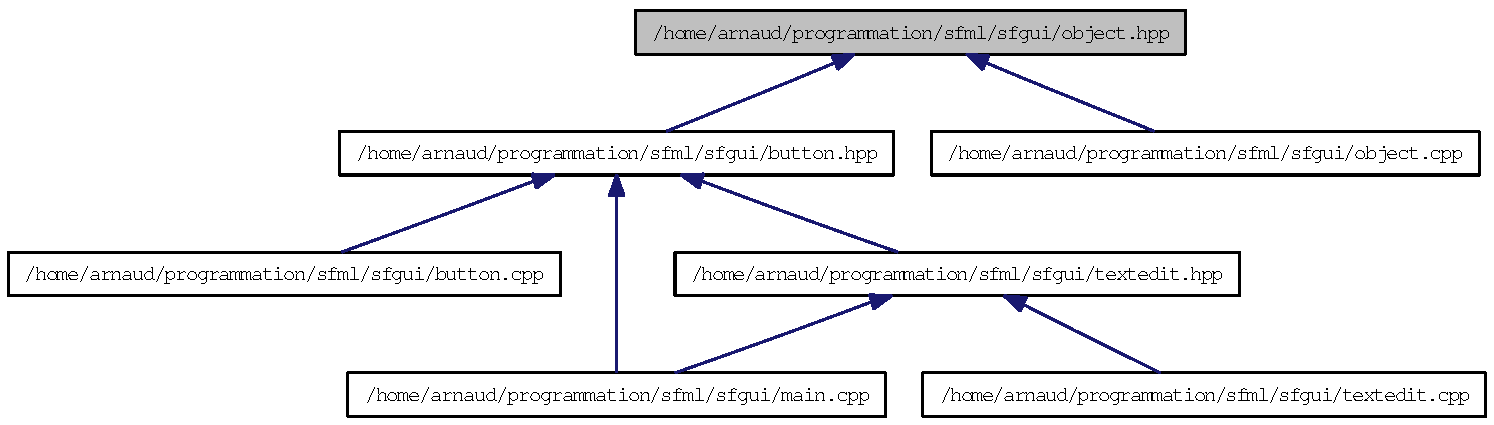
\includegraphics[width=420pt]{object_8hpp__dep__incl}
\end{center}
\end{figure}
\subsection*{Namespaces}
\begin{CompactItemize}
\item 
namespace \hyperlink{namespacesfgui}{sfgui}
\end{CompactItemize}
\subsection*{Classes}
\begin{CompactItemize}
\item 
class \hyperlink{classsfgui_1_1Object}{sfgui::Object}
\begin{CompactList}\small\item\em A simple graphic item. \item\end{CompactList}\end{CompactItemize}

\hypertarget{textedit_8cpp}{
\section{/home/arnaud/programmation/sfml/sfgui/textedit.cpp File Reference}
\label{textedit_8cpp}\index{/home/arnaud/programmation/sfml/sfgui/textedit.cpp@{/home/arnaud/programmation/sfml/sfgui/textedit.cpp}}
}
{\tt \#include \char`\"{}textedit.hpp\char`\"{}}\par


Include dependency graph for textedit.cpp:\nopagebreak
\begin{figure}[H]
\begin{center}
\leavevmode
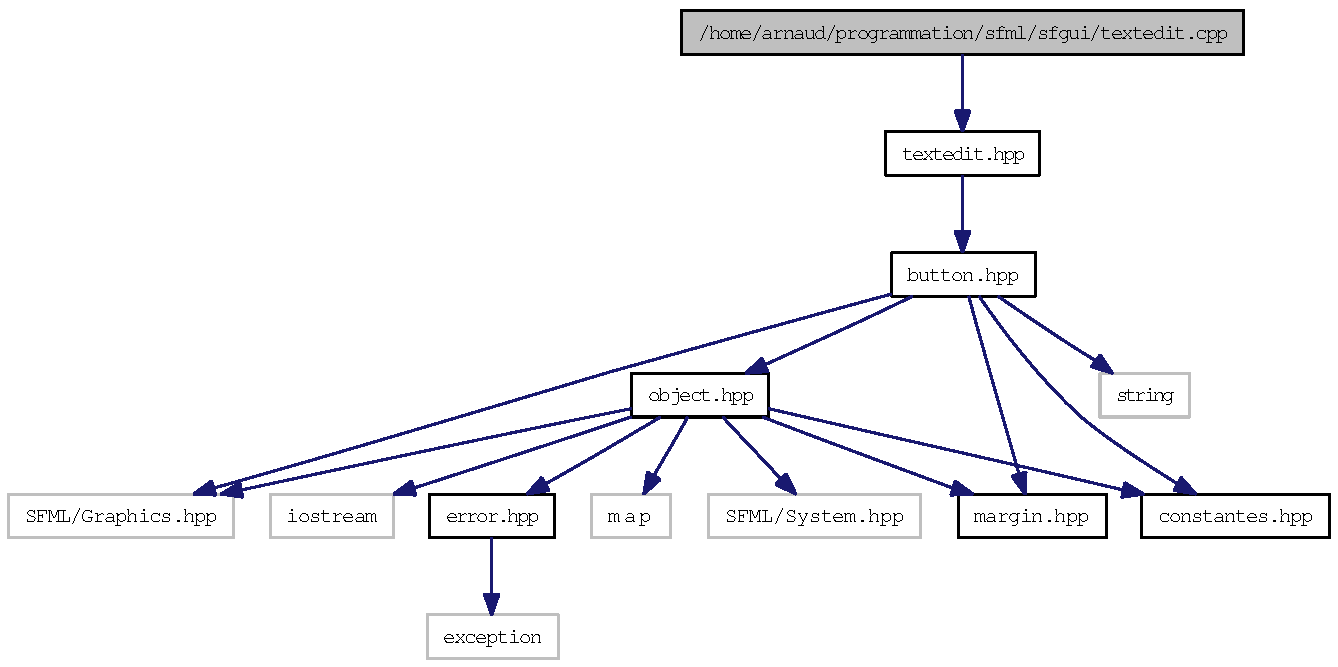
\includegraphics[width=339pt]{textedit_8cpp__incl}
\end{center}
\end{figure}

\hypertarget{textedit_8hpp}{
\section{/home/arnaud/programmation/sfml/sfgui/textedit.hpp File Reference}
\label{textedit_8hpp}\index{/home/arnaud/programmation/sfml/sfgui/textedit.hpp@{/home/arnaud/programmation/sfml/sfgui/textedit.hpp}}
}
{\tt \#include \char`\"{}button.hpp\char`\"{}}\par


Include dependency graph for textedit.hpp:\nopagebreak
\begin{figure}[H]
\begin{center}
\leavevmode
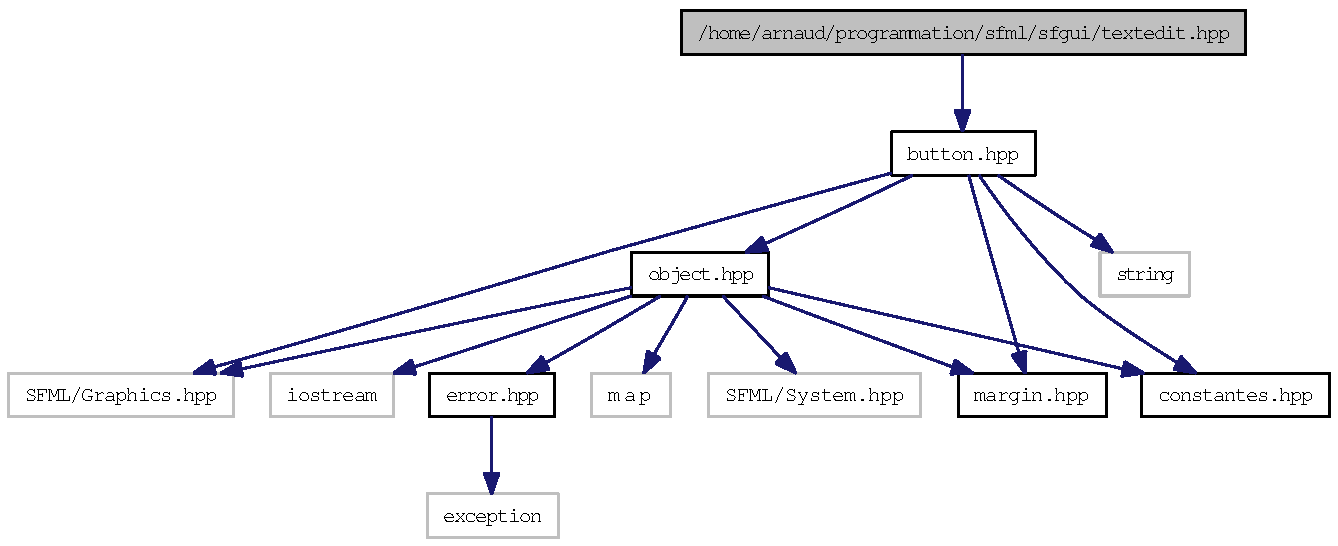
\includegraphics[width=339pt]{textedit_8hpp__incl}
\end{center}
\end{figure}


This graph shows which files directly or indirectly include this file:\nopagebreak
\begin{figure}[H]
\begin{center}
\leavevmode
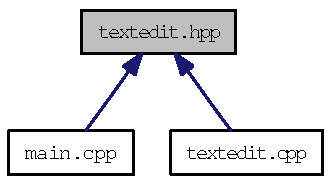
\includegraphics[width=295pt]{textedit_8hpp__dep__incl}
\end{center}
\end{figure}
\subsection*{Namespaces}
\begin{CompactItemize}
\item 
namespace \hyperlink{namespacesfgui}{sfgui}
\end{CompactItemize}
\subsection*{Classes}
\begin{CompactItemize}
\item 
class \hyperlink{classsfgui_1_1TextEdit}{sfgui::TextEdit}
\begin{CompactList}\small\item\em A single line text entry. \item\end{CompactList}\end{CompactItemize}

\printindex
\end{document}
